\section{Results}
\label{sec:results}

\begin{itemize}
	\item Irradiation worsens electrical properties of silicon sensors.
	\item Bulk-dominated leakage current per volumne expected to increase proportionally with fluence, investigated in~\ref{subsec:irradiation_alpha}.
	\item Depletion voltage expected to increase, shown in~\ref{subsec:irradiation_Vdep}.		
	\item Characterisation measurements discussed here are before after additional annealing
	\item Annealing, i.e. heating up, during long shutdowns
	\item \SI{80}{\minute} at \SI{60}{\celsius} corresponds to xx at yy or cc at bb (best-case scenario)
	\item Characterisation measurements discussed here performed at \SI{-40}{\celsius} and at very low humidity
	\item Overall: Characteristics as expected after irradiation, and after annealing
\end{itemize}

\subsection{Leakage Current}
\label{subsec:leakagecurrents}

\begin{figure}
	\captionsetup[subfigure]{aboveskip=-1pt,belowskip=-1pt}
	\centering
	\begin{subfigure}[b]{0.49\textwidth}
		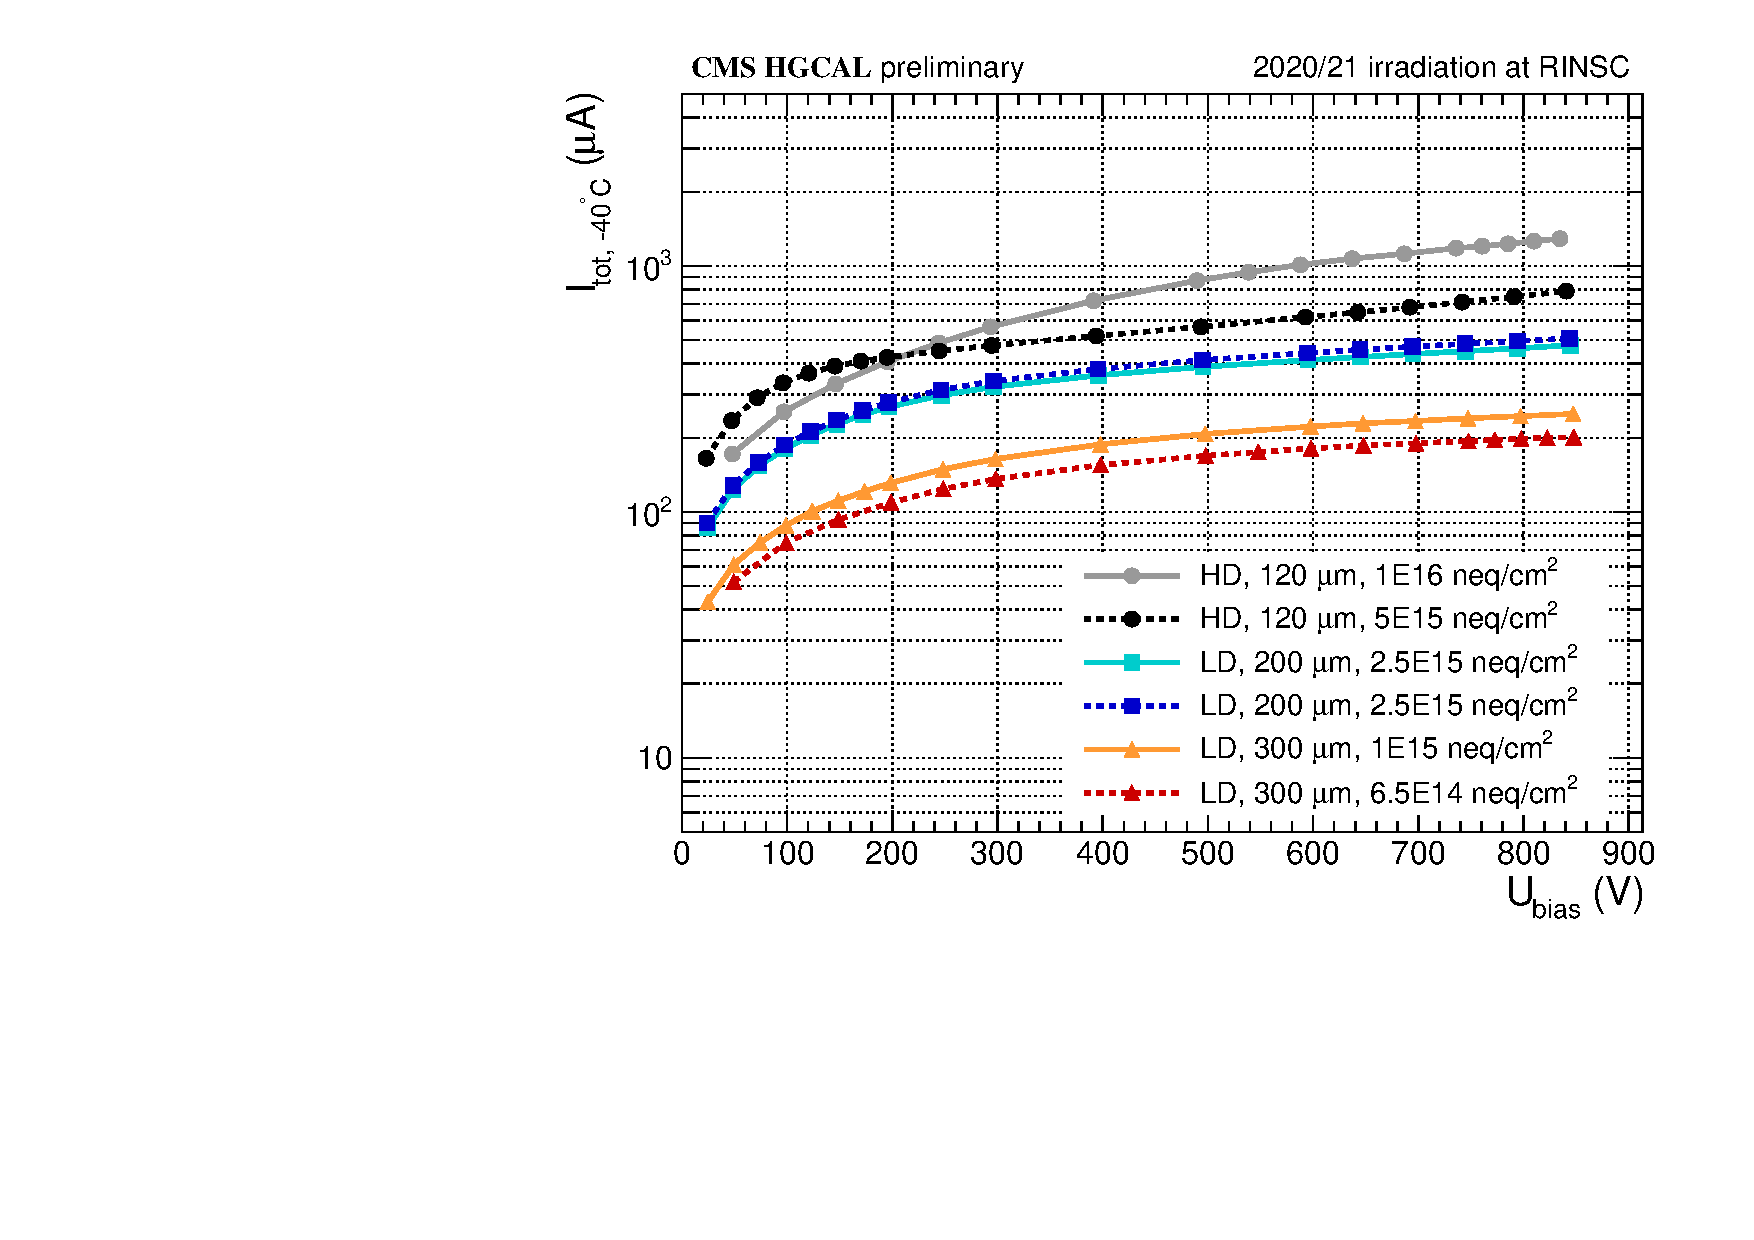
\includegraphics[width=0.999\textwidth]{plots/total_iv/total_current_IV.pdf}
		\subcaption{
		}
		\label{plot:tot_IV_good}
    \end{subfigure}
    \hfill
    \begin{subfigure}[b]{0.49\textwidth}
        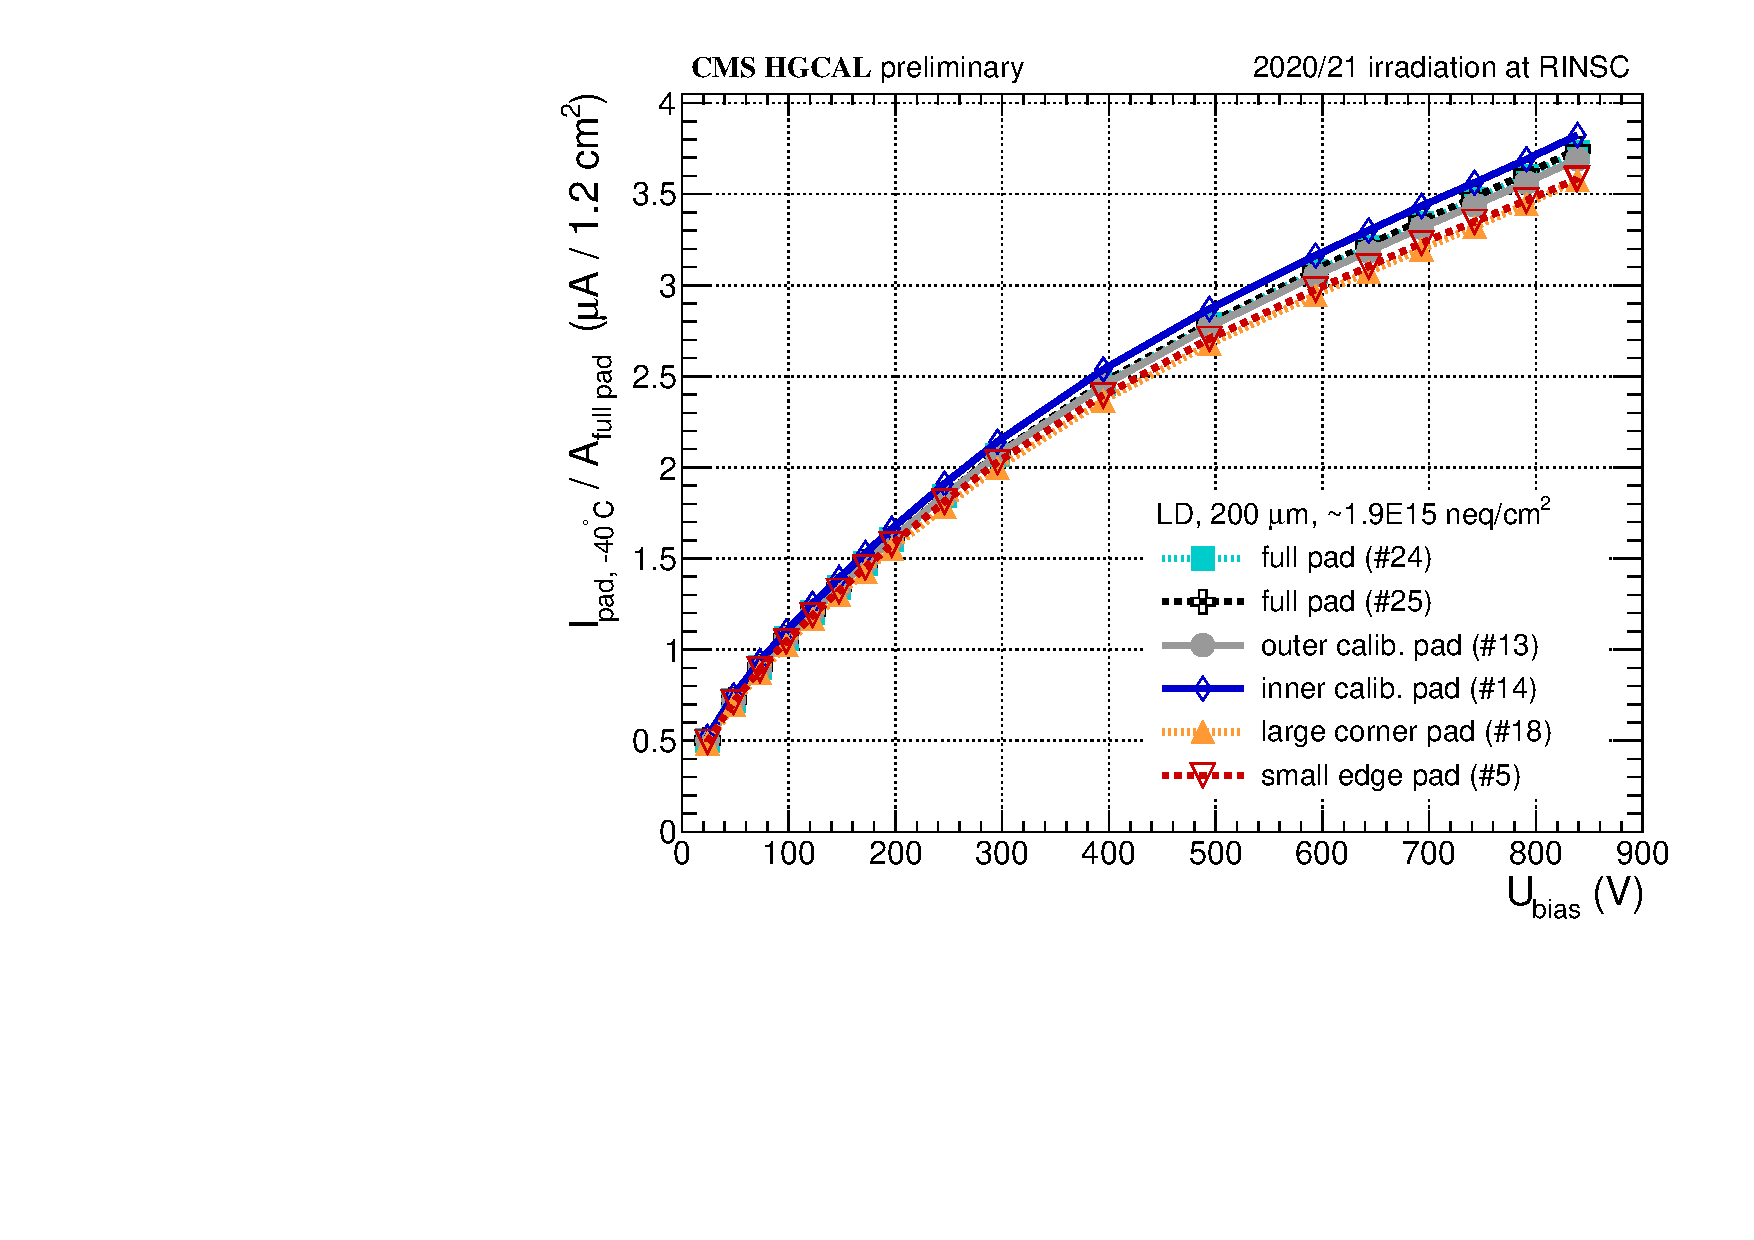
\includegraphics[width=0.999\textwidth]{plots/channel_iv/channel_IV_sensors_channels.pdf}
        \subcaption{
        }
        \label{plot:pad_IV_channels}
    \end{subfigure}

	\caption{
		(a) Total leakage currents after irradiation (without additional annealing) for two representative example sensors. 
		Currents were measured at \SI{-40}{\celsius} ($\text{I}_\text{tot, \SI{-40}{\celsius}}$) and at different effective bias voltages ($\text{U}_\text{bias}$). 
        (b) Per-pad leakage currents normalised to the area of full hexagonal pads as a function of the effective bias voltage for different pads with different geometries on one example sensor.
	}
\end{figure}

The total leakage current is defined as the current flowing through R$_\text{HV}$ in \ref{fig:switchprobecard_CAD} and can be understood as the dark current of a full silicon wafer.
As it is exemplified for two prototype sensors in \ref{plot:tot_IV_good}, the total leakage current did not exhibit exponential growth and stayed well below the ARRAY system compliance of \SI{2}{\milli\ampere} for most of the irradiated sensors that were tested up to \SI{850}{\volt} at \SI{-40}{\celsius}.
Irreversible discharges occurred only for a handful of the tested sensors.
There, the total leakage current during electrical characterisation suddenly increased and exceeded the \SI{2}{\milli\ampere} limitation.
Whereas one half of those instances could be traced back to pre-existing conditions such as mechanical damages induced during the irradiation or the transport, the other half lead to a design modification of the HGCAL silicon sensors which should minimise the risk of discharges in the future\footnote{More than 20 prototype sensors with the improved design have been characterized with voltages up to \SI{850}{\volt} in the meantime. None have shown discharges thus far.}.
Results of the affected sensors are not discussed further in this section.\newline
\ref{plot:pad_IV_channels} shows the per-pad leakage current as a function of the effective bias voltage (\emph{IV}) for adjacent pads on one representative sensor irradiated to intermediate fluences.
In general, our data demonstrate that the leakage current of a pad after irradiation scales with its volume, and that the relative increase from \SI{600}{\volt} to \SI{800}{\volt} remains well below \SI{150}{\percent}.

\begin{figure}
	\captionsetup[subfigure]{aboveskip=-1pt,belowskip=-1pt}
	\centering
	\begin{subfigure}[b]{0.49\textwidth}
		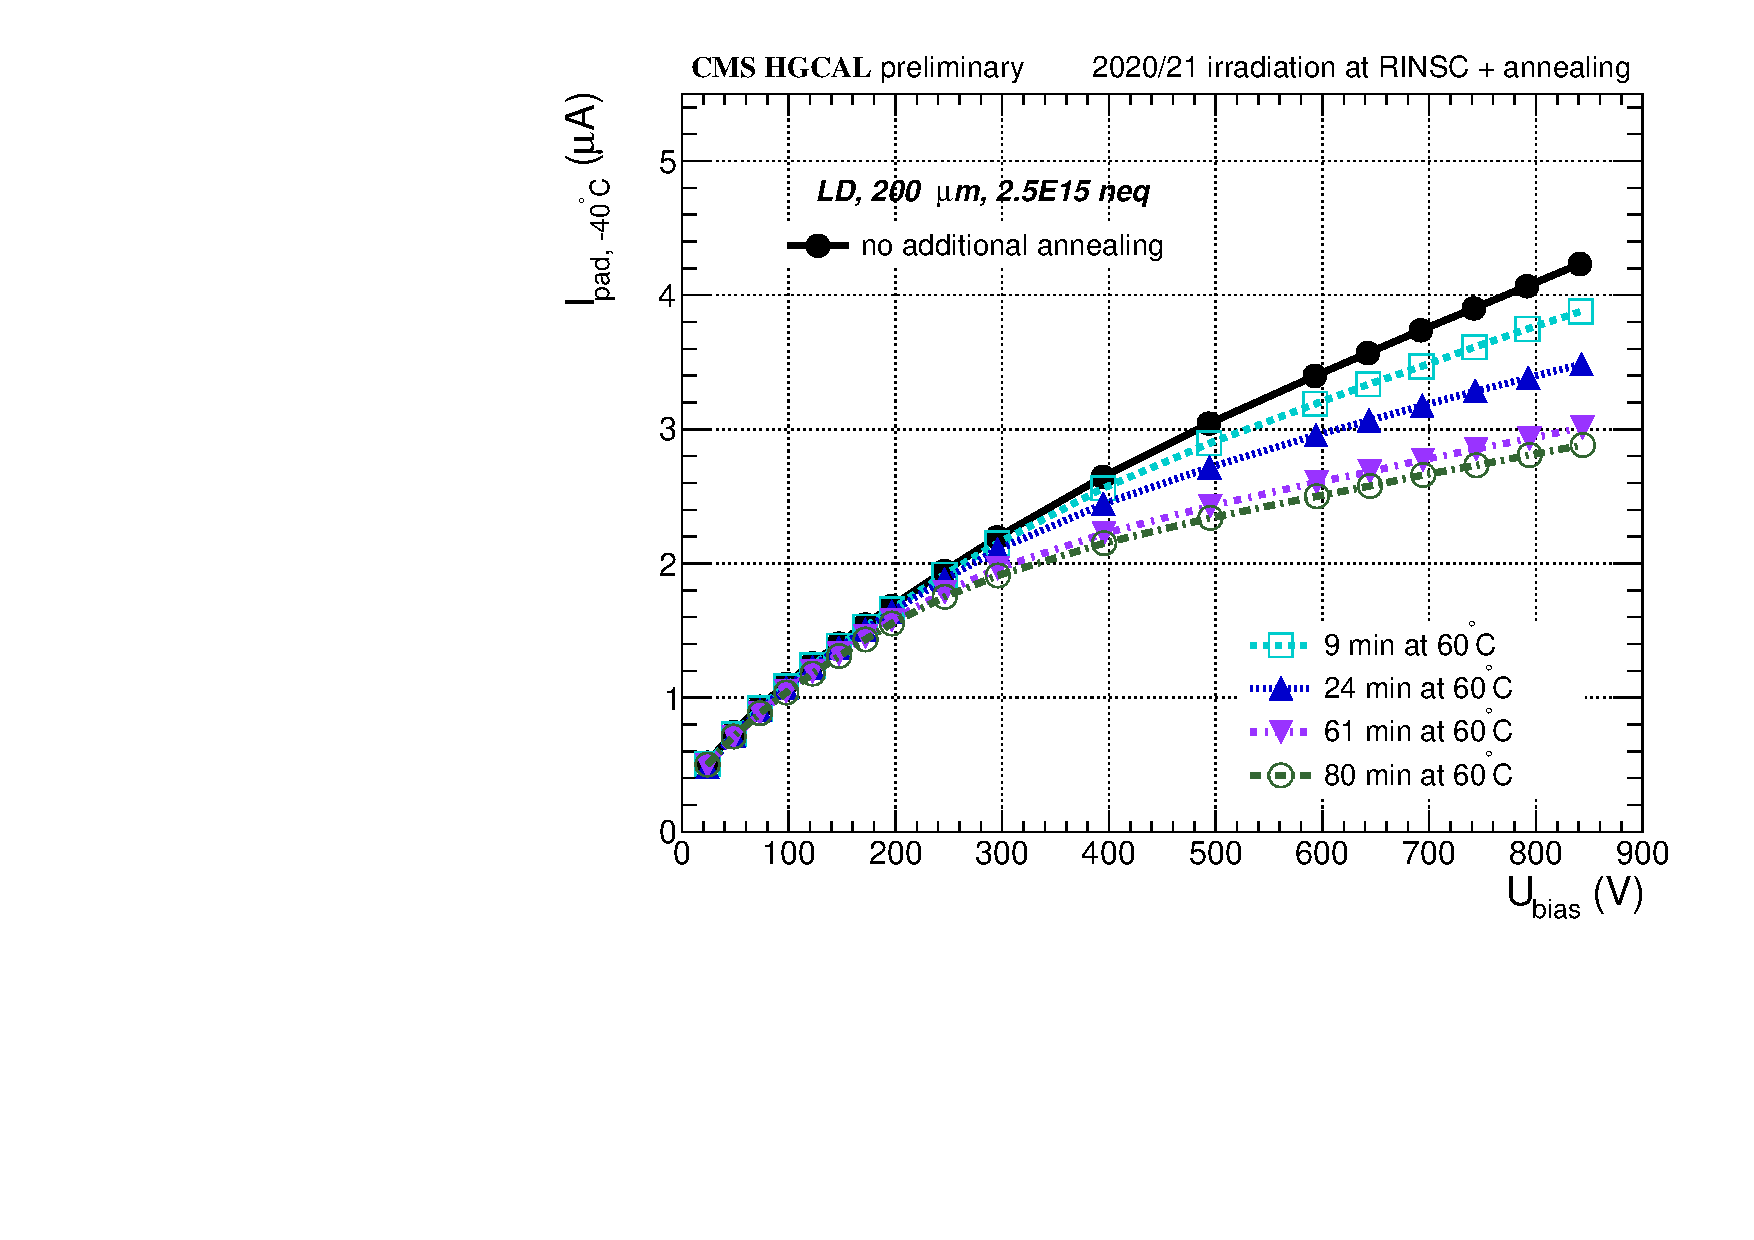
\includegraphics[width=0.999\textwidth]{plots/annealing_iv/annealing_IV_ch24.pdf}
		\subcaption{
		}
		\label{plot:annealing_IV}
	\end{subfigure}
	\hfill
	\begin{subfigure}[b]{0.49\textwidth}
		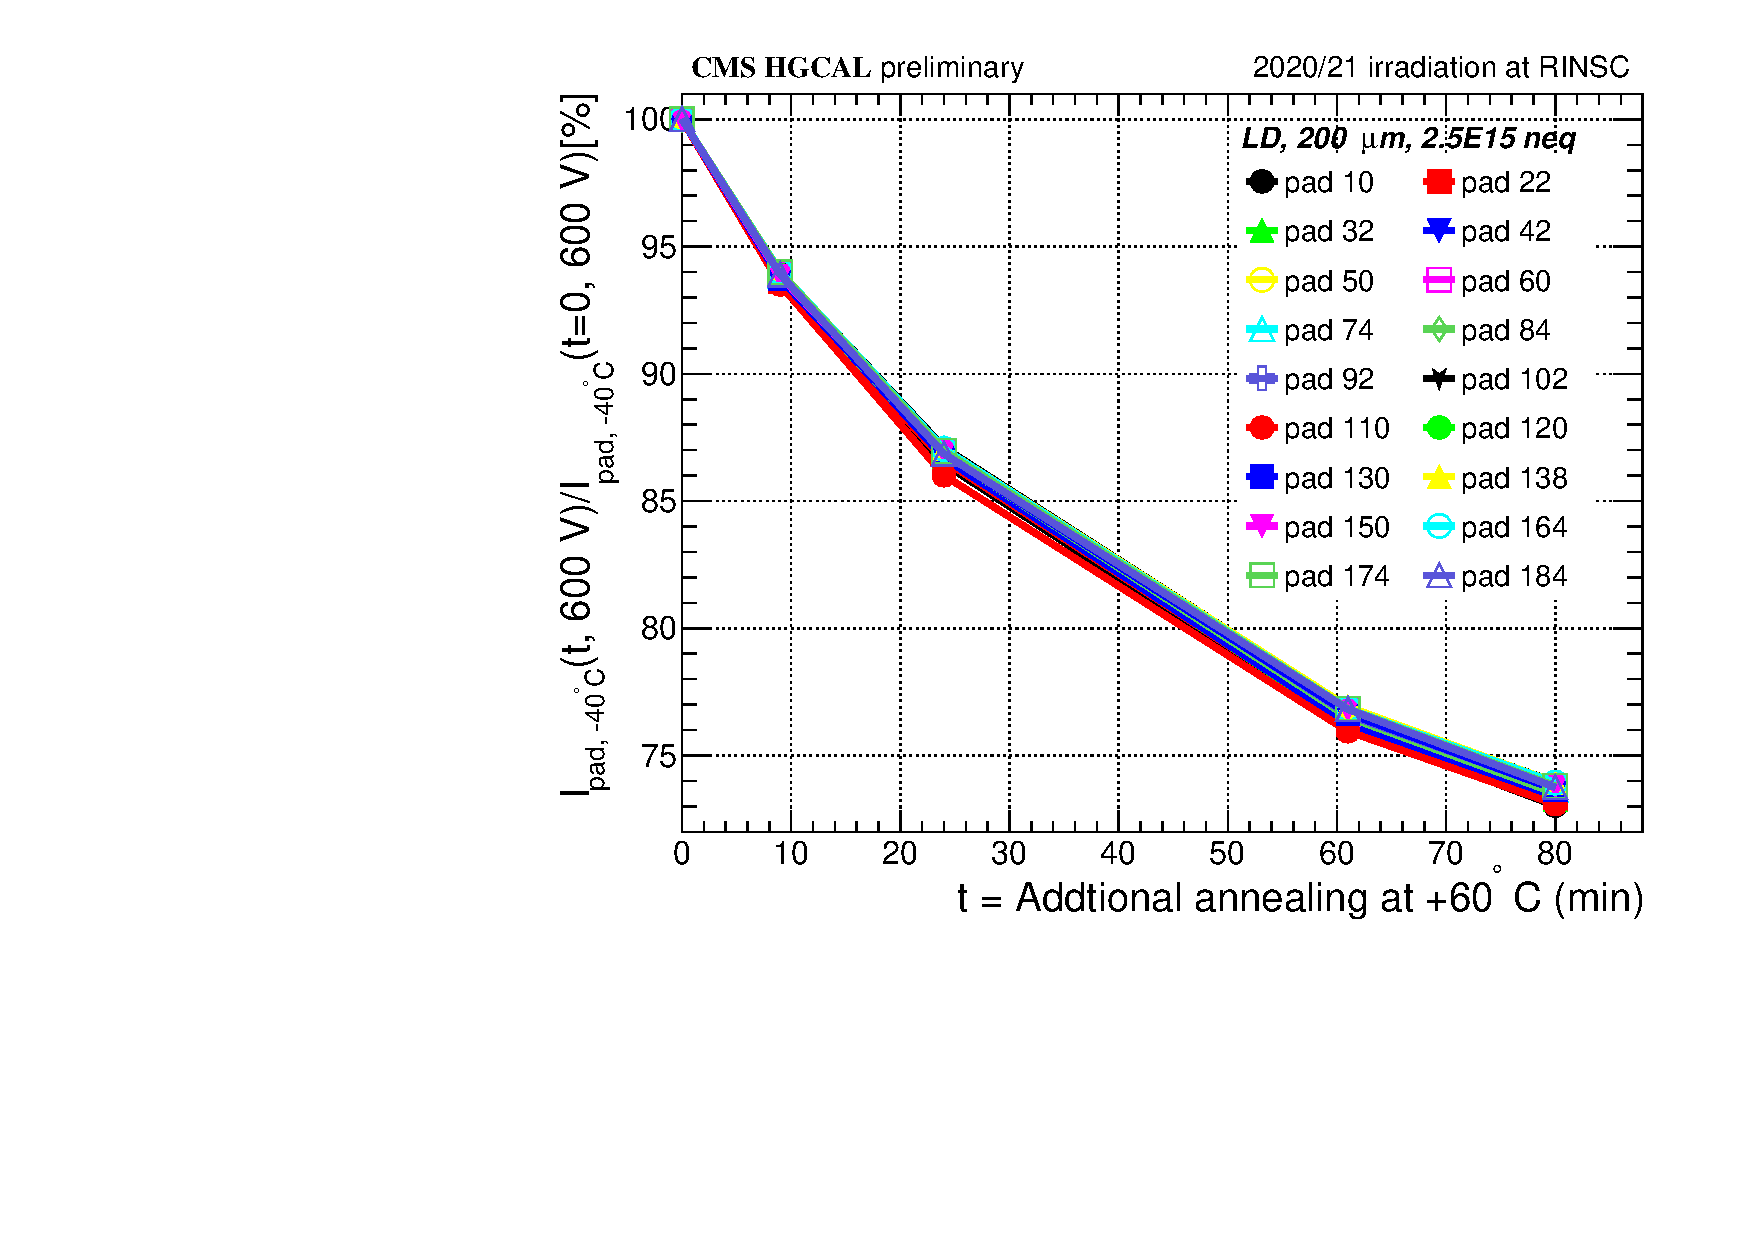
\includegraphics[width=0.999\textwidth]{plots/annealing_iv/annealing_current.pdf}
		\subcaption{
		}
		\label{plot:annealing_current}
	\end{subfigure}    

	\caption{
		(a) IV-curves of a representative full hexagonal pad for different annealing scenarios for a \SI{200}{\micro\metre} low-density prototype sensor irradiated to approximately 2.4$~$E15 1-MeV-neutron equivalents/cm$^{2}$.
        (b) Decrease of the per-pad leakage current (interpolated to $U_\text{bias}=U_\text{dep}$) as a function of the additional annealing time at \SI{60}{\celsius} for a subset of full hexagonal pads.
	}
\end{figure}

\begin{itemize}
	\item \ref{plot:annealing_IV}: illustrate the improvement in leakage current with annealing (study a sensor with minimal additional annealing during irradiation)
	\item IV curves lowered especially at high bias voltages beyond full depletion where bulk currents dominate
	\item Note that current at \SI{600}{\volt} reduced by approximately 25$~\%$ for all pads after \SI{80}{\min}
	\item Benefitting from both leakage current decrease and depletion voltage decrease = \ref{plot:annealing_current}: Current at depletion voltage reduced by approximately 35$~\%$ for all pads
\end{itemize}





\begin{figure}
	\captionsetup[subfigure]{aboveskip=-1pt,belowskip=-1pt}
	\centering
	\begin{subfigure}[b]{0.32\textwidth}
		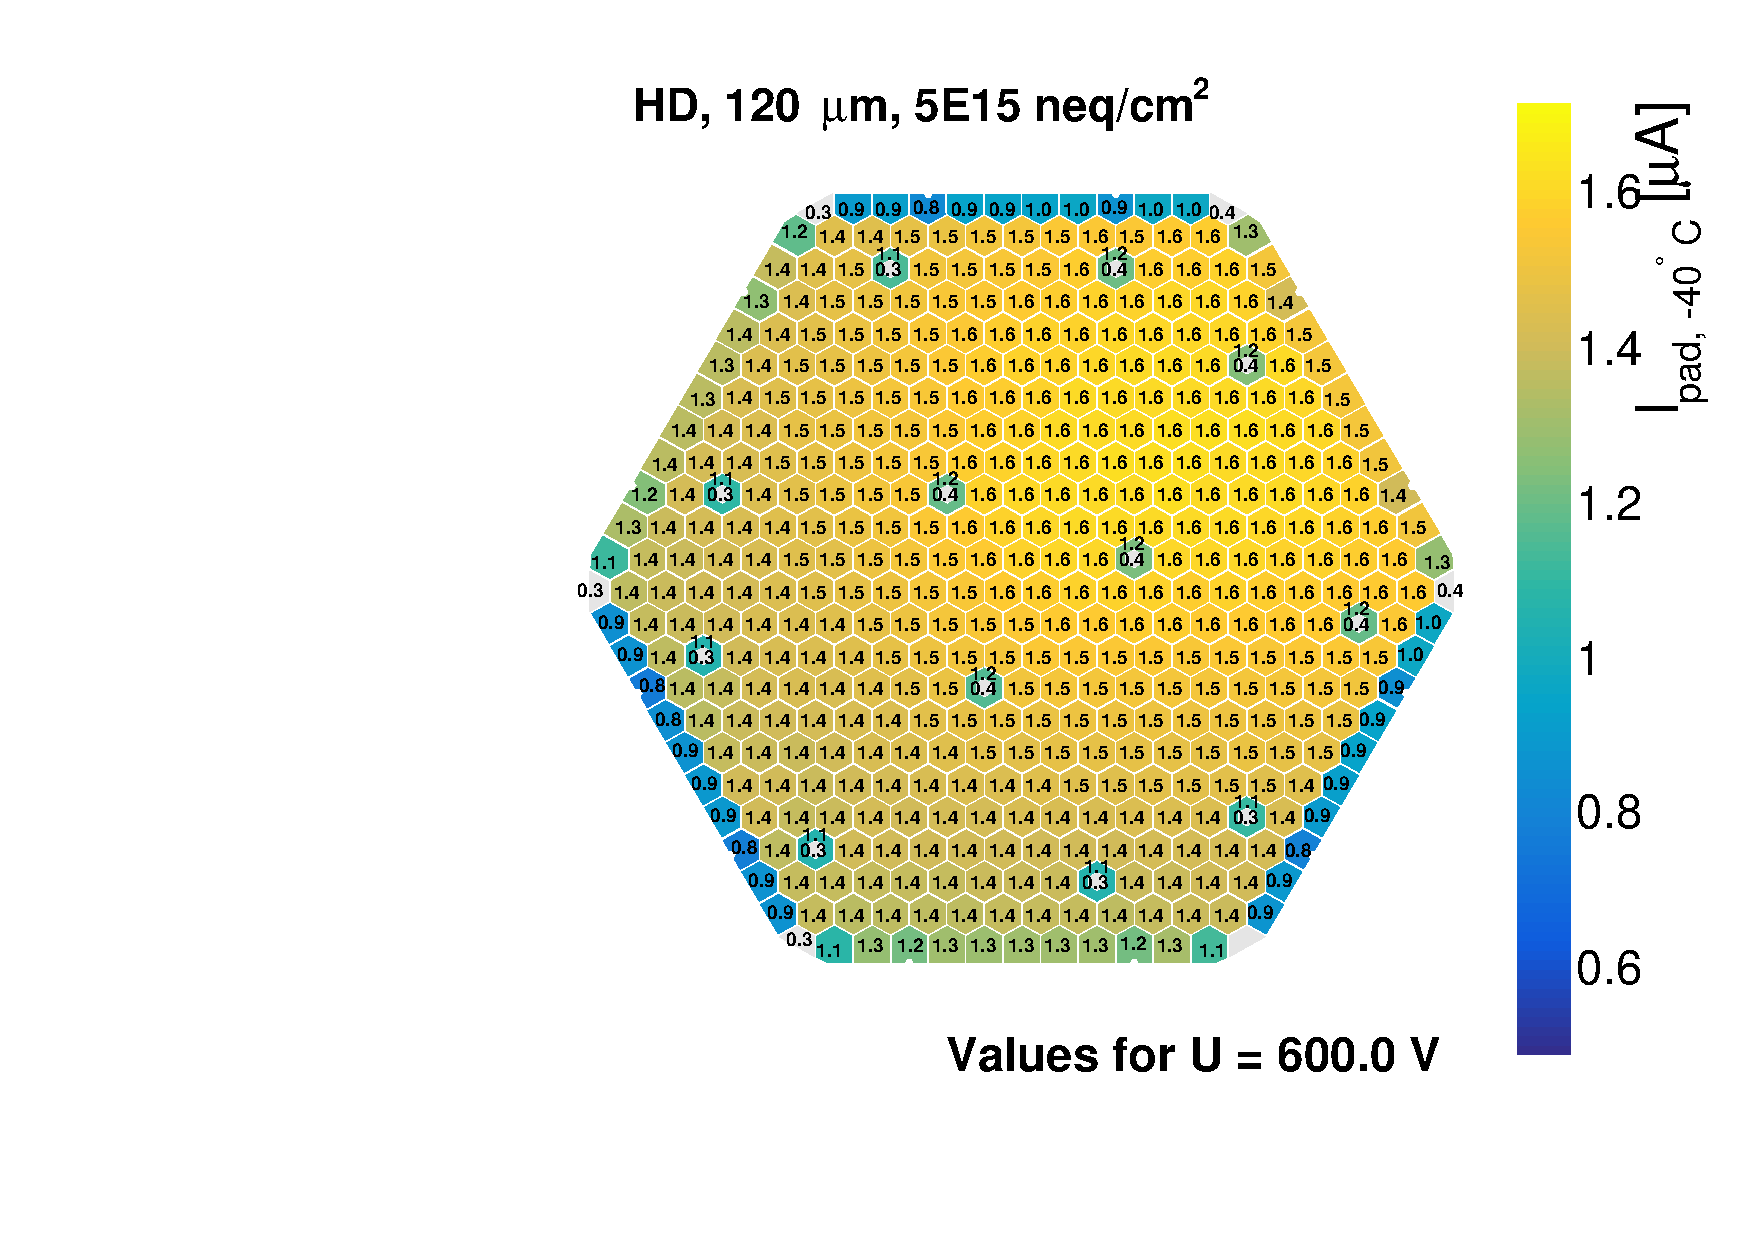
\includegraphics[width=0.999\textwidth]{plots/iv_hexplots/3009.pdf}
		\subcaption{
		}
		\label{plot:iv_hexplot_3009}
	\end{subfigure}
	\hfill
	\begin{subfigure}[b]{0.32\textwidth}
		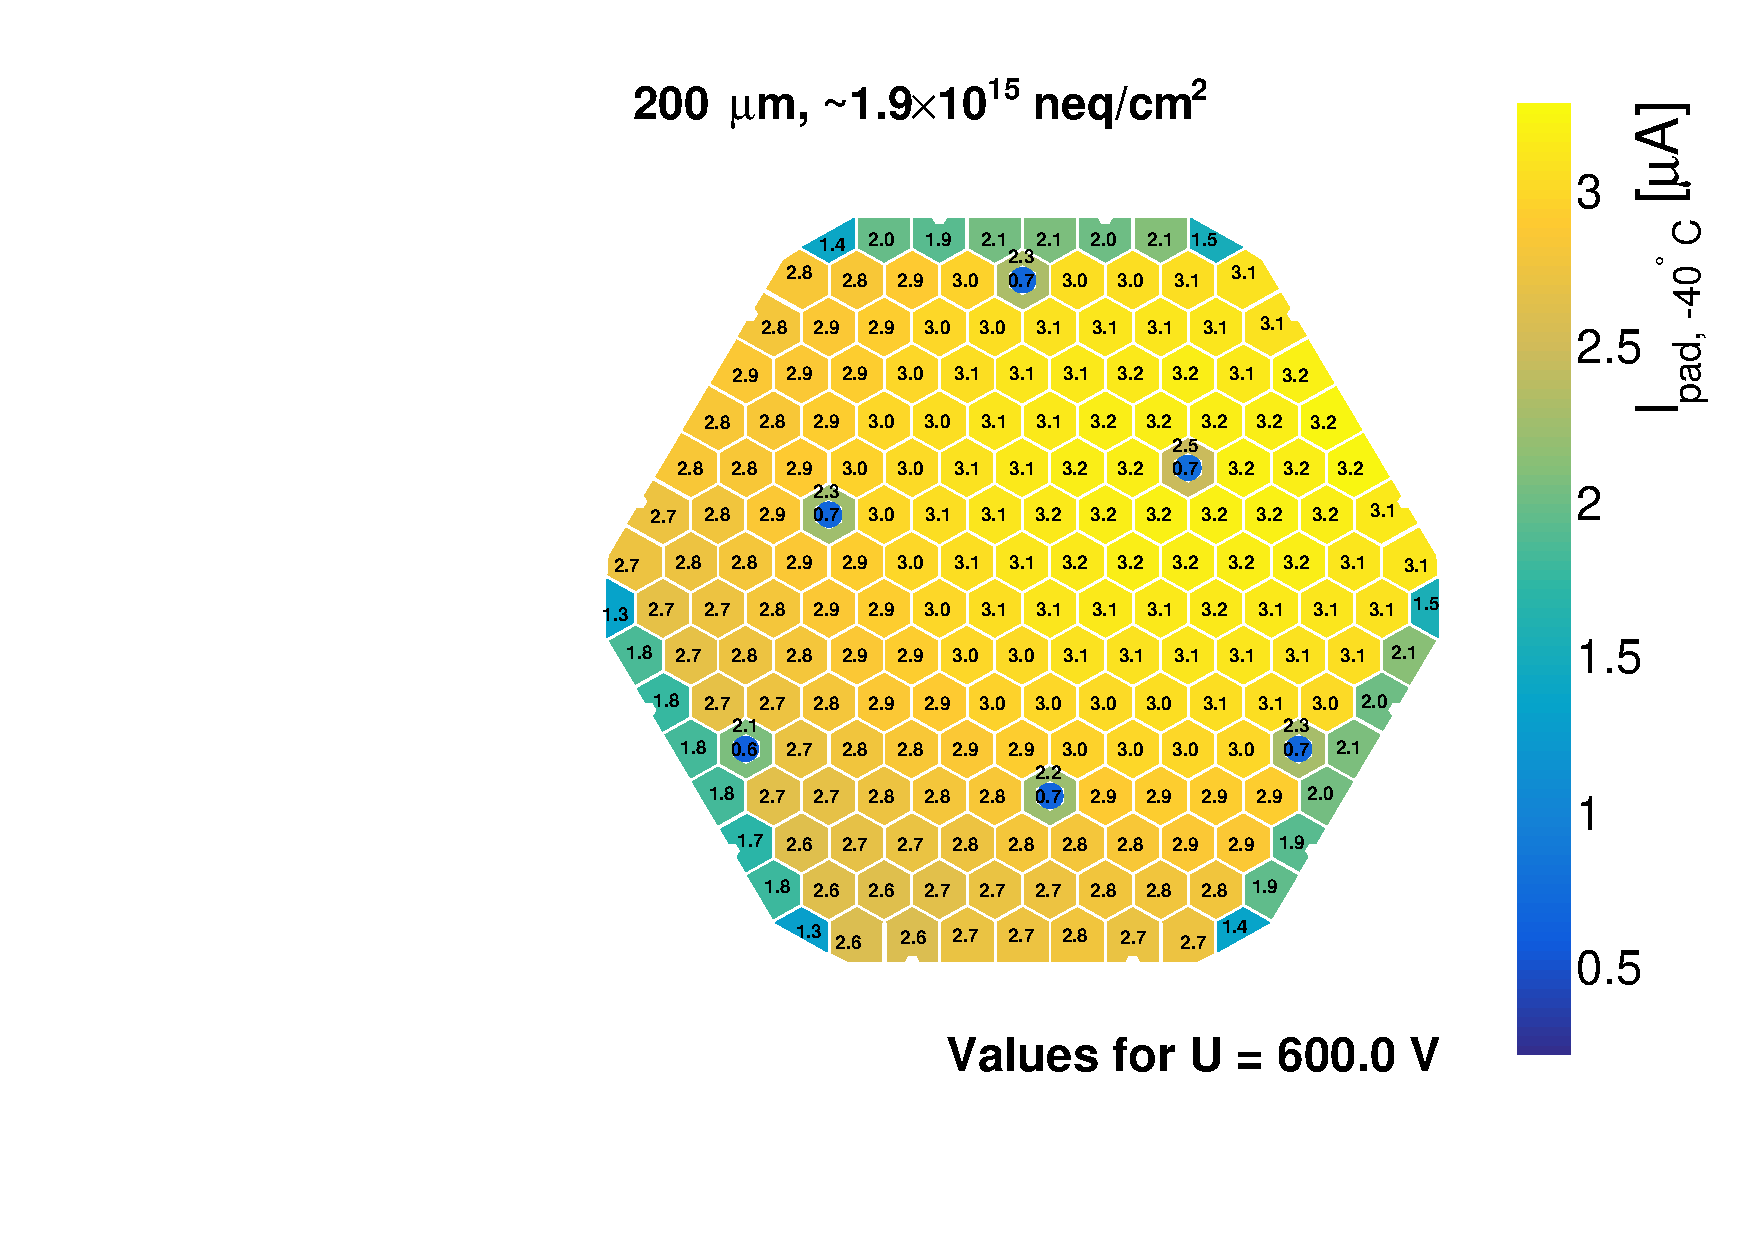
\includegraphics[width=0.999\textwidth]{plots/iv_hexplots/0541_04.pdf}
		\subcaption{
		}
		\label{plot:iv_hexplot_0541_04}
	\end{subfigure}
	\hfill	
	\begin{subfigure}[b]{0.32\textwidth}
		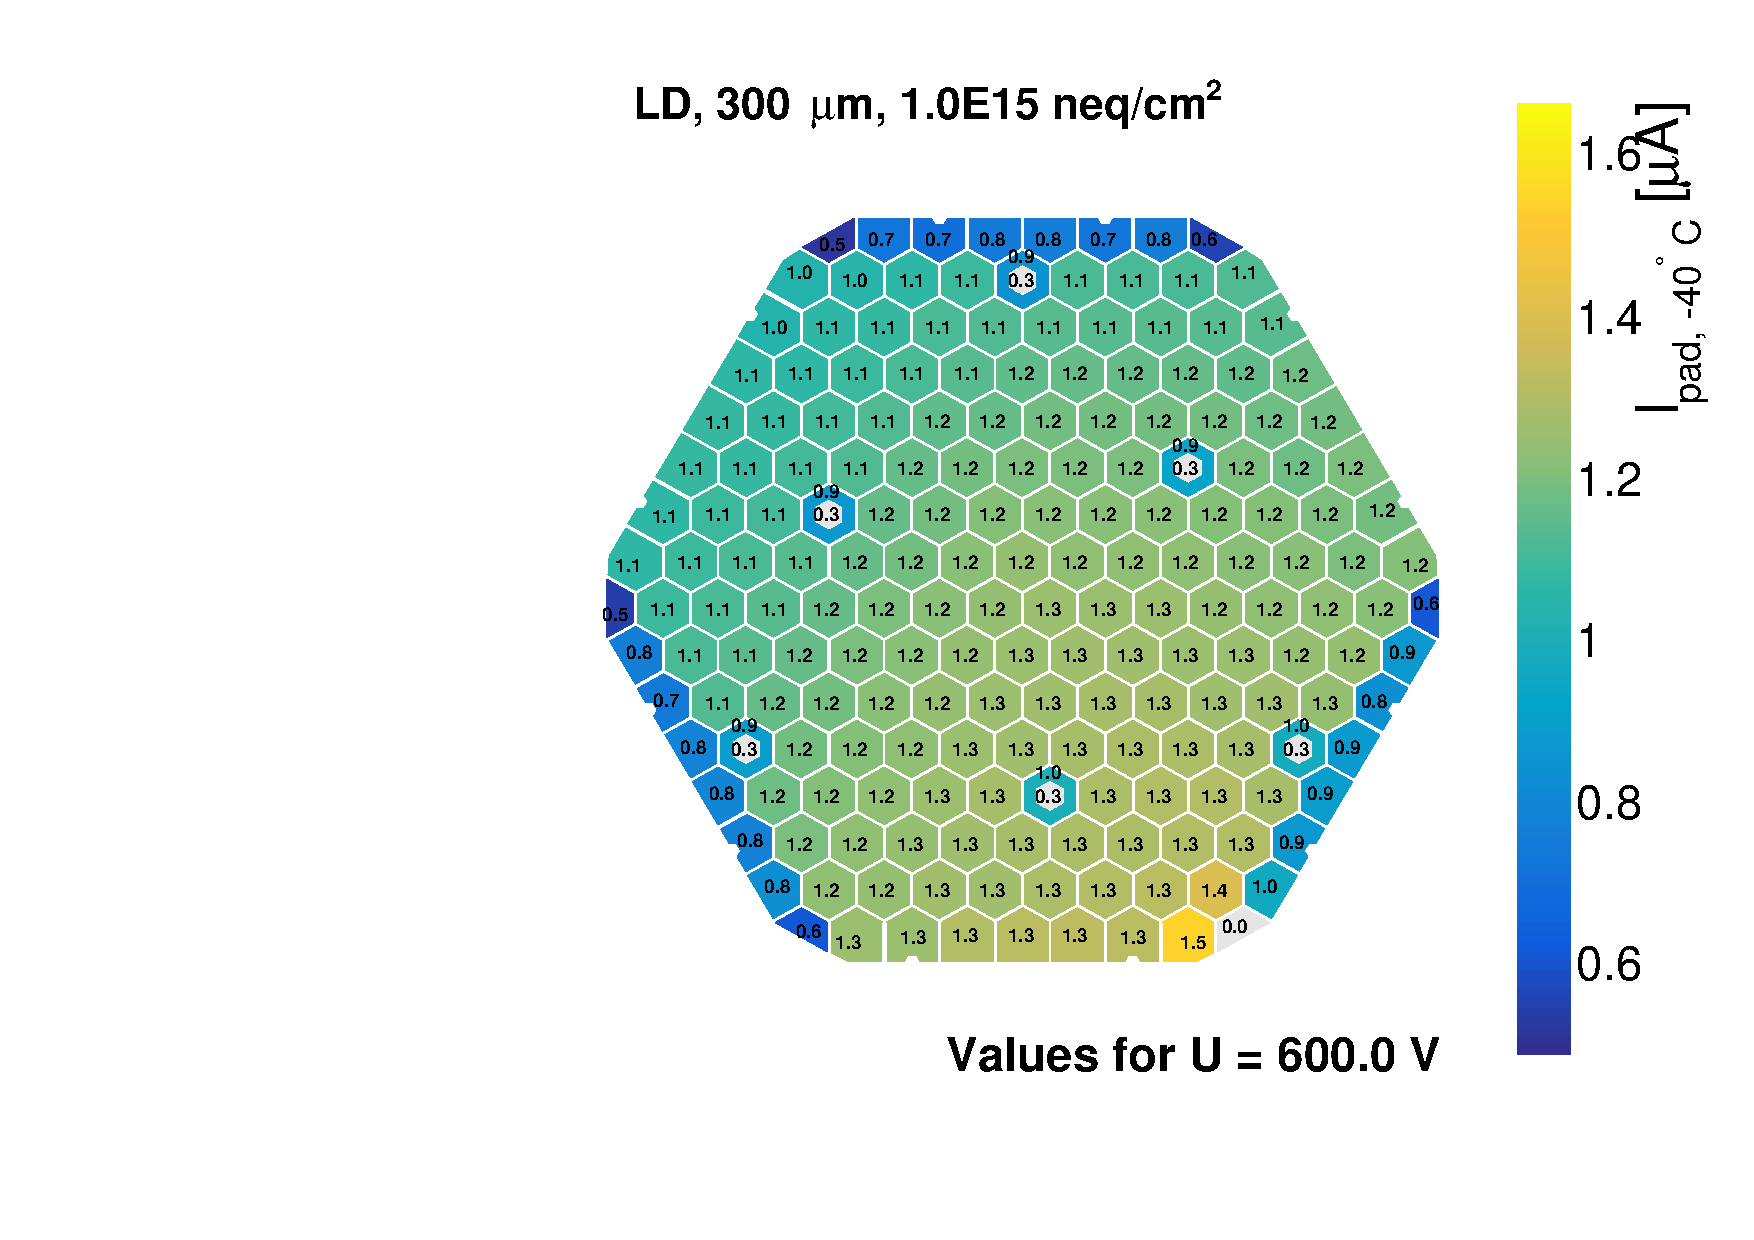
\includegraphics[width=0.999\textwidth]{plots/iv_hexplots/1013.pdf}
		\subcaption{
		}
		\label{plot:iv_hexplot_1013}
	\end{subfigure}
    \hfill
	\begin{subfigure}[b]{0.32\textwidth}
		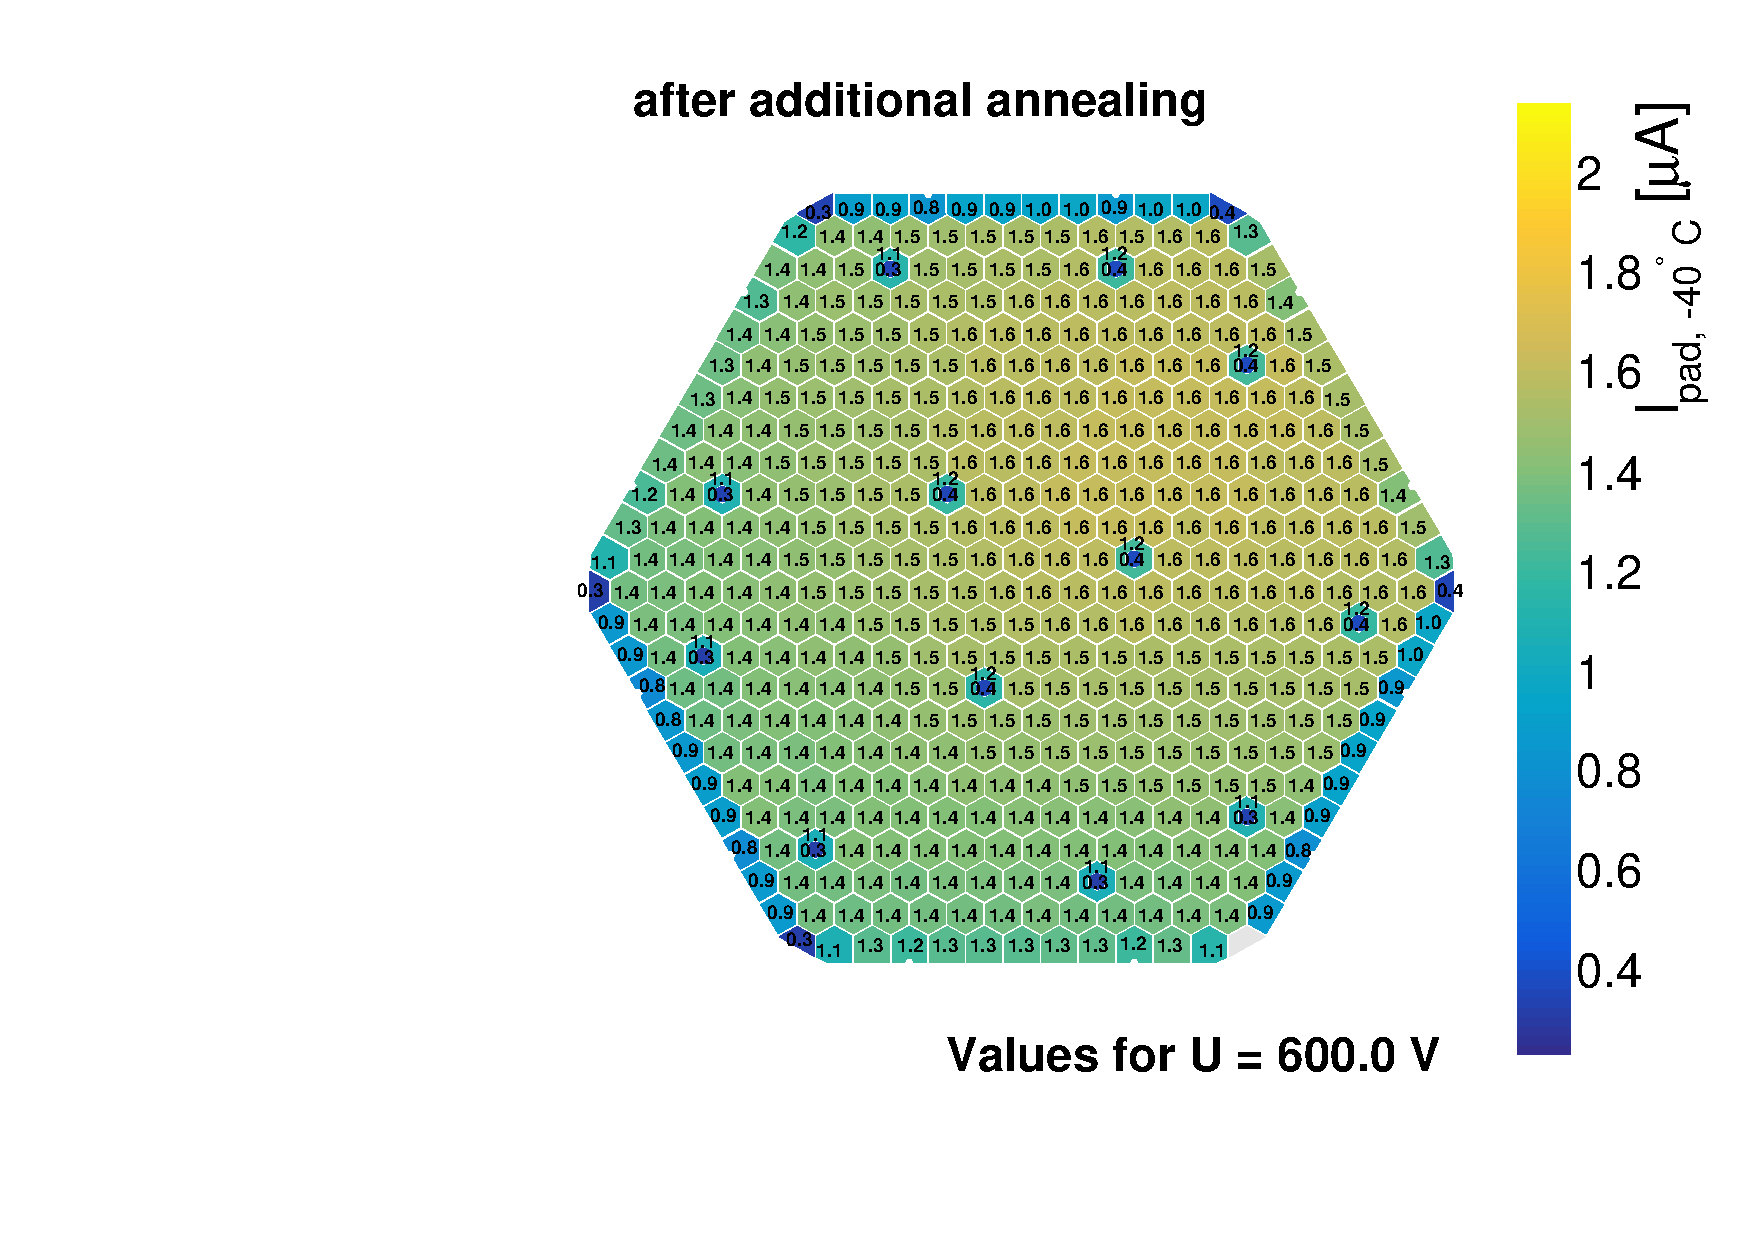
\includegraphics[width=0.999\textwidth]{plots/iv_hexplots/3009_annealed.pdf}
		\subcaption{
		}
		\label{plot:iv_hexplot_3009_annealed}
	\end{subfigure}
	\hfill
	\begin{subfigure}[b]{0.32\textwidth}
		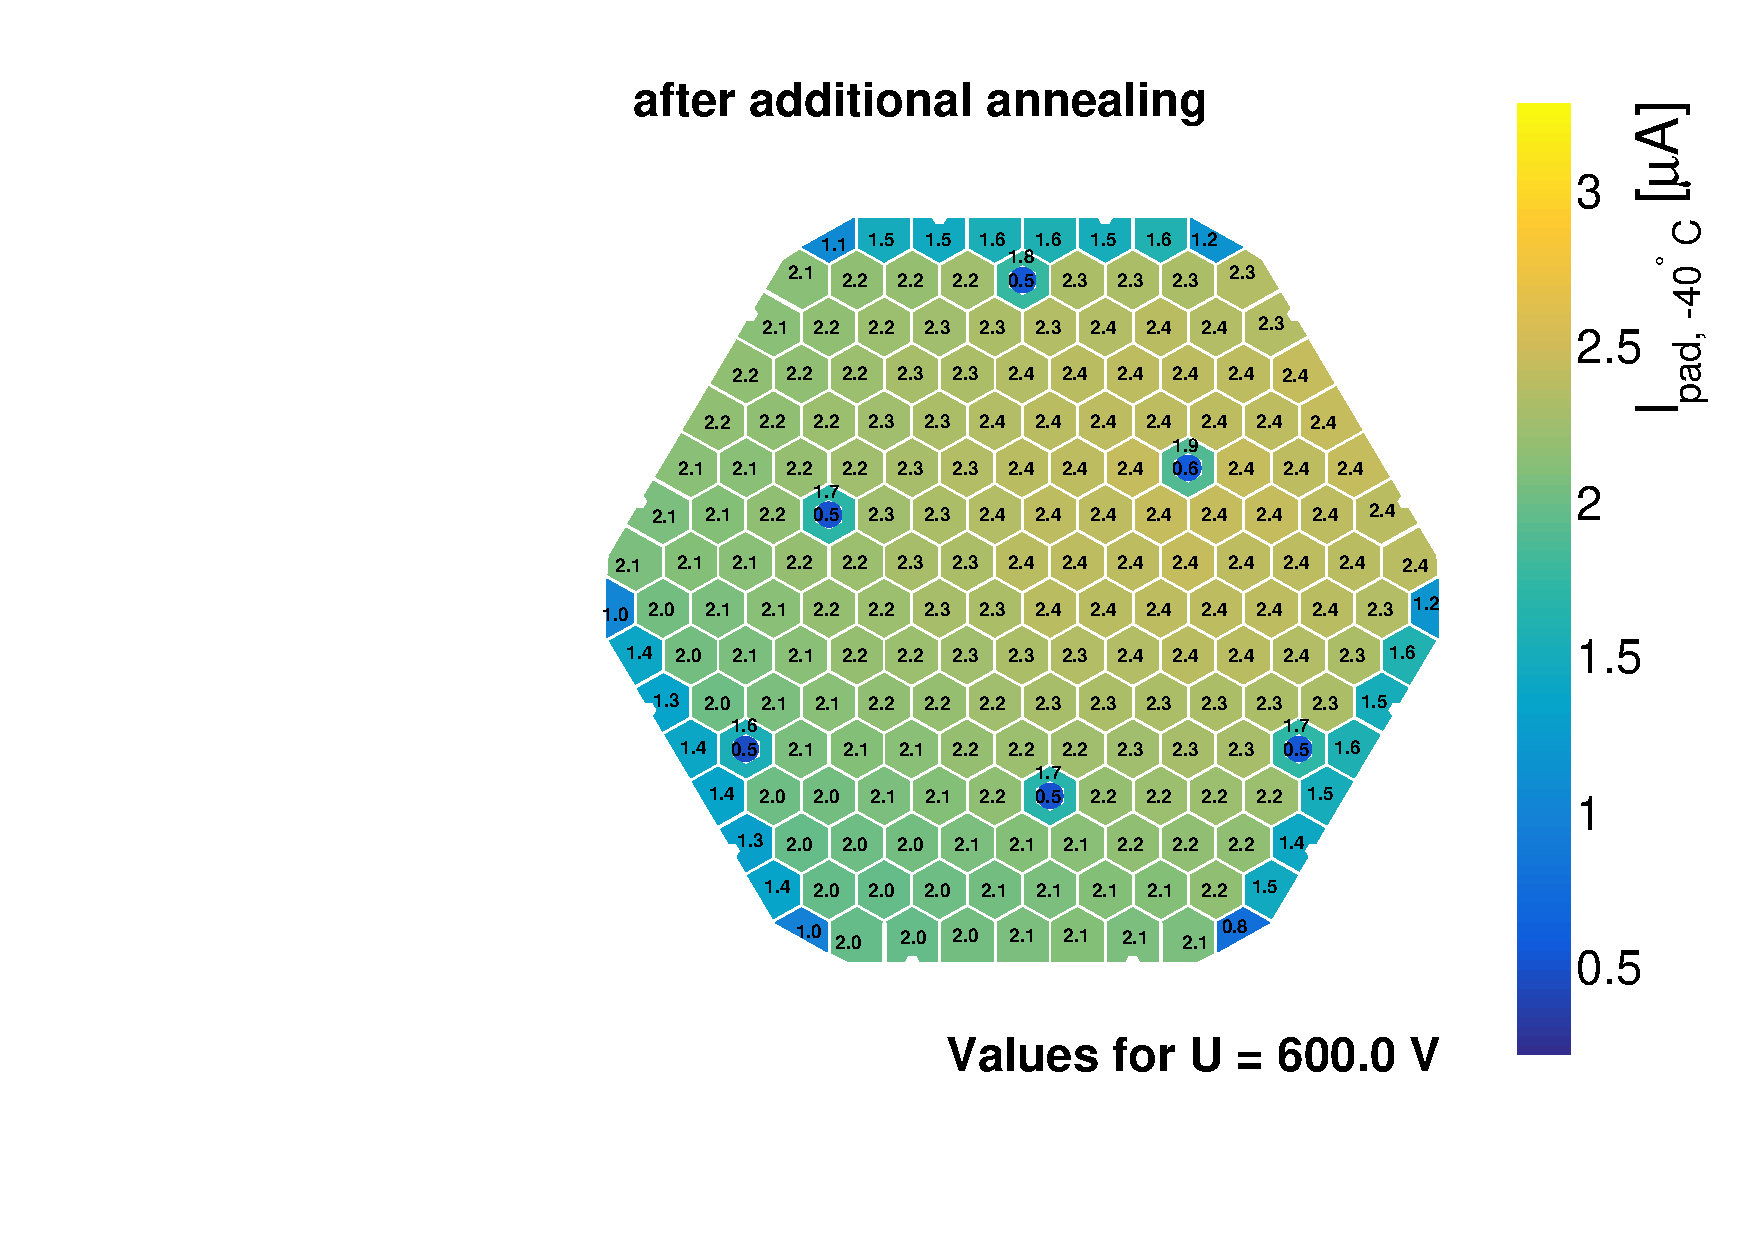
\includegraphics[width=0.999\textwidth]{plots/iv_hexplots/0541_04_annealed.pdf}
		\subcaption{
		}
		\label{plot:iv_hexplot_0541_04_annealed}
	\end{subfigure}
	\hfill	
	\begin{subfigure}[b]{0.32\textwidth}
		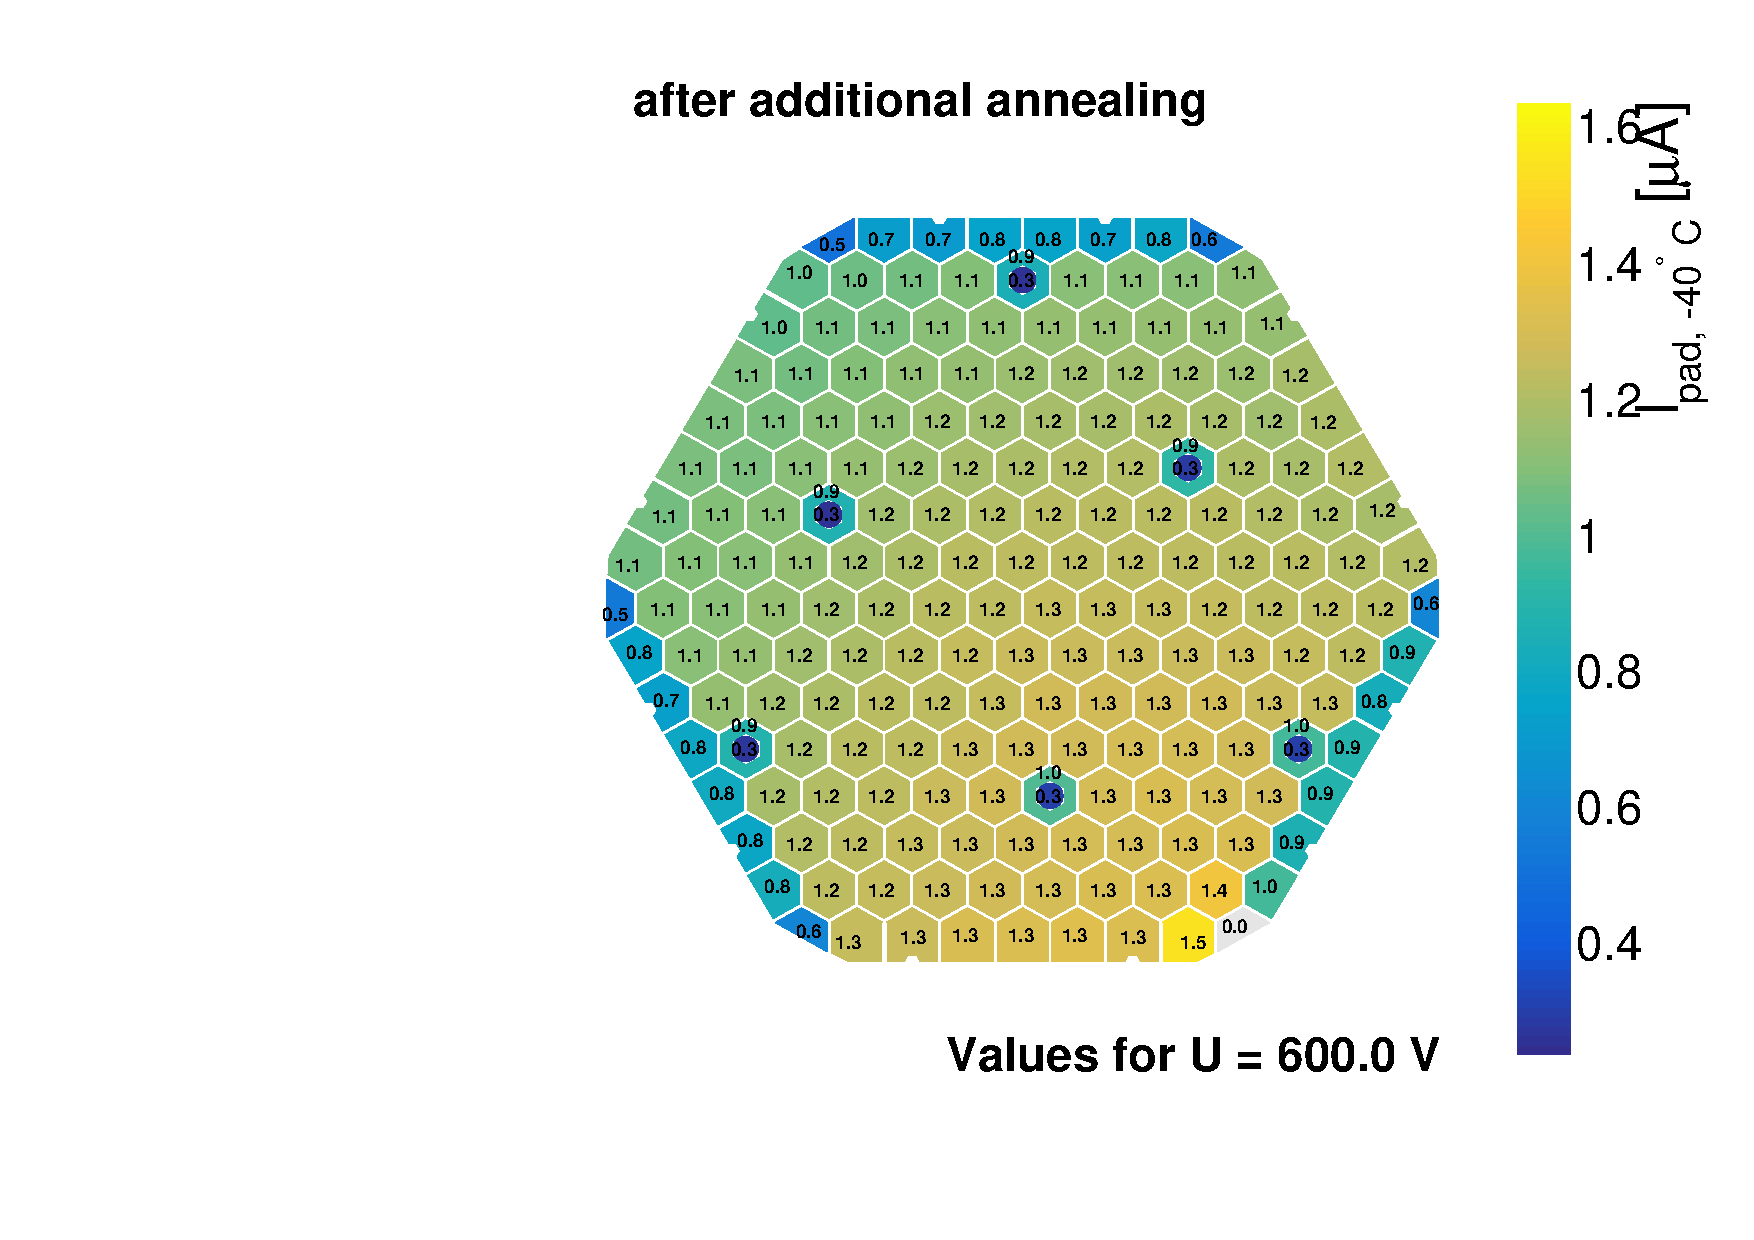
\includegraphics[width=0.999\textwidth]{plots/iv_hexplots/1013_annealed.pdf}
		\subcaption{
		}
		\label{plot:iv_hexplot_1013_annealed}
	\end{subfigure}    
	\label{plot:iv_hexplot}
	\caption{
		Per-pad leakage currents interpolated to an effective bias voltage of \SI{600}{\volt} for three representative sensors from different irradiation rounds before (a-c) and after additional annealing (d-e).
		The chuck temperature profile is corrected for, cf.~\ref{appendix:chuck_temp}.
		Red- or white-colored edge pads correspond to well-understood (however undesired) measurement peculiarities, e.g. unconnected pogo pins.
		Note the different leakage current colour scales.
	}
\end{figure}

\begin{itemize}
	\item Per-pad currents interpolated to \SI{600}{\volt} for representative good sensors shown in~\ref{plot:iv_hexplot_3003,plot:iv_hexplot_3009,plot:iv_hexplot_0541_04,plot:iv_hexplot_2004,plot:iv_hexplot_1013,plot:iv_hexplot_1002}
	\item Provide table of approximate leakage currents
	\item Profile is visible, is attributed to fluence profile
\end{itemize}


\begin{figure}
	\captionsetup[subfigure]{aboveskip=-1pt,belowskip=-1pt}
	\centering
    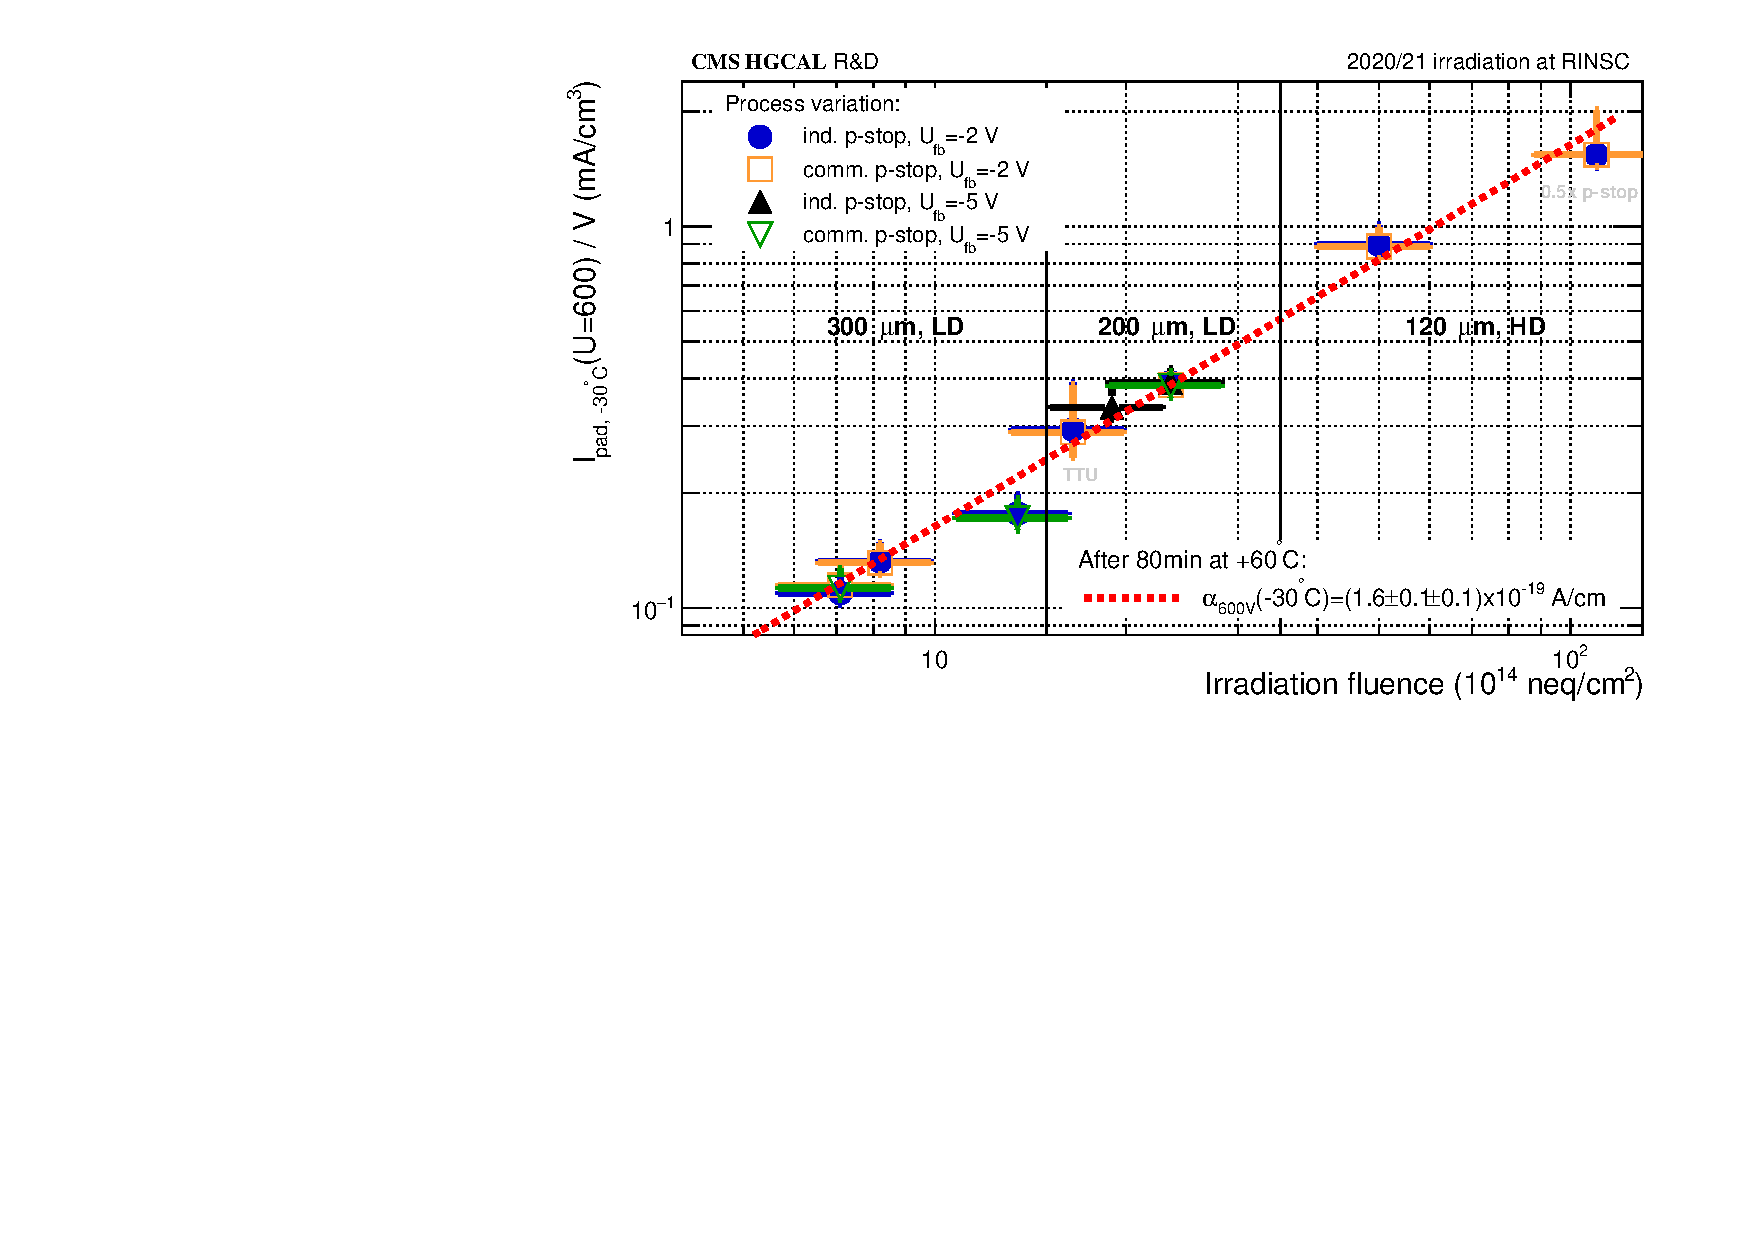
\includegraphics[width=0.69\textwidth]{plots/alpha/alpha_600V.pdf}
    \label{plot:alpha_600}
	\caption{
	    Volume-normalised per-pad leakage current for different fluences at a bias voltage of \SI{600}{\volt}.
        Prototype sensors were characterised after additional annnealing at \SI{60}{\celsius} at CERN and at Texas Tech University (TTU).
		Measured leakage currents are scaled to a room-temperature of \SI{+20}{\celsius}.
        The current-relate damage rate ($\alpha$) is found to be independent of the sensor production parameters investigated in this work.
	}
\end{figure}

\begin{itemize}
	\item Leakage currents normalised by volume, scaled to \SI{-20}{\celsius}, cf.~\ref{eq:temp_scaling}
	\item Observe: Proportionality, constant referred to as $\alpha$, cf.~\ref{plot:alpha_Udep,plot:alpha_600}
	\item Report three different alpha values: one around full depletion, one at \SI{600}{\volt} and the third at highest bias voltage of \SI{800}{\volt} (corresponding to end of HGCAL lifetime)
	\item Observe: Independence on sensor production parameters, consistent with previous findings, e.g.~\cite{moll:SiDamages}
	\item All $\alpha$ constants underestimated, w.r.t. literature values, fluence monitoring not yet satisfactory yet.
\end{itemize}


\subsection{Capacitance and Depletion Voltage}
\label{subsec:Udep}
\begin{itemize}
	\item Capacitances are open-corrected, serial definition, LCR frequency = 2kHz (reminder)
	\item Systematic measurements of capacitances after annealing only --> limitations (should not be used for extrapolation to CMS scenario)
\end{itemize}


\begin{figure}
	\captionsetup[subfigure]{aboveskip=-1pt,belowskip=-1pt}
	\centering

	\begin{subfigure}[b]{0.49\textwidth}
		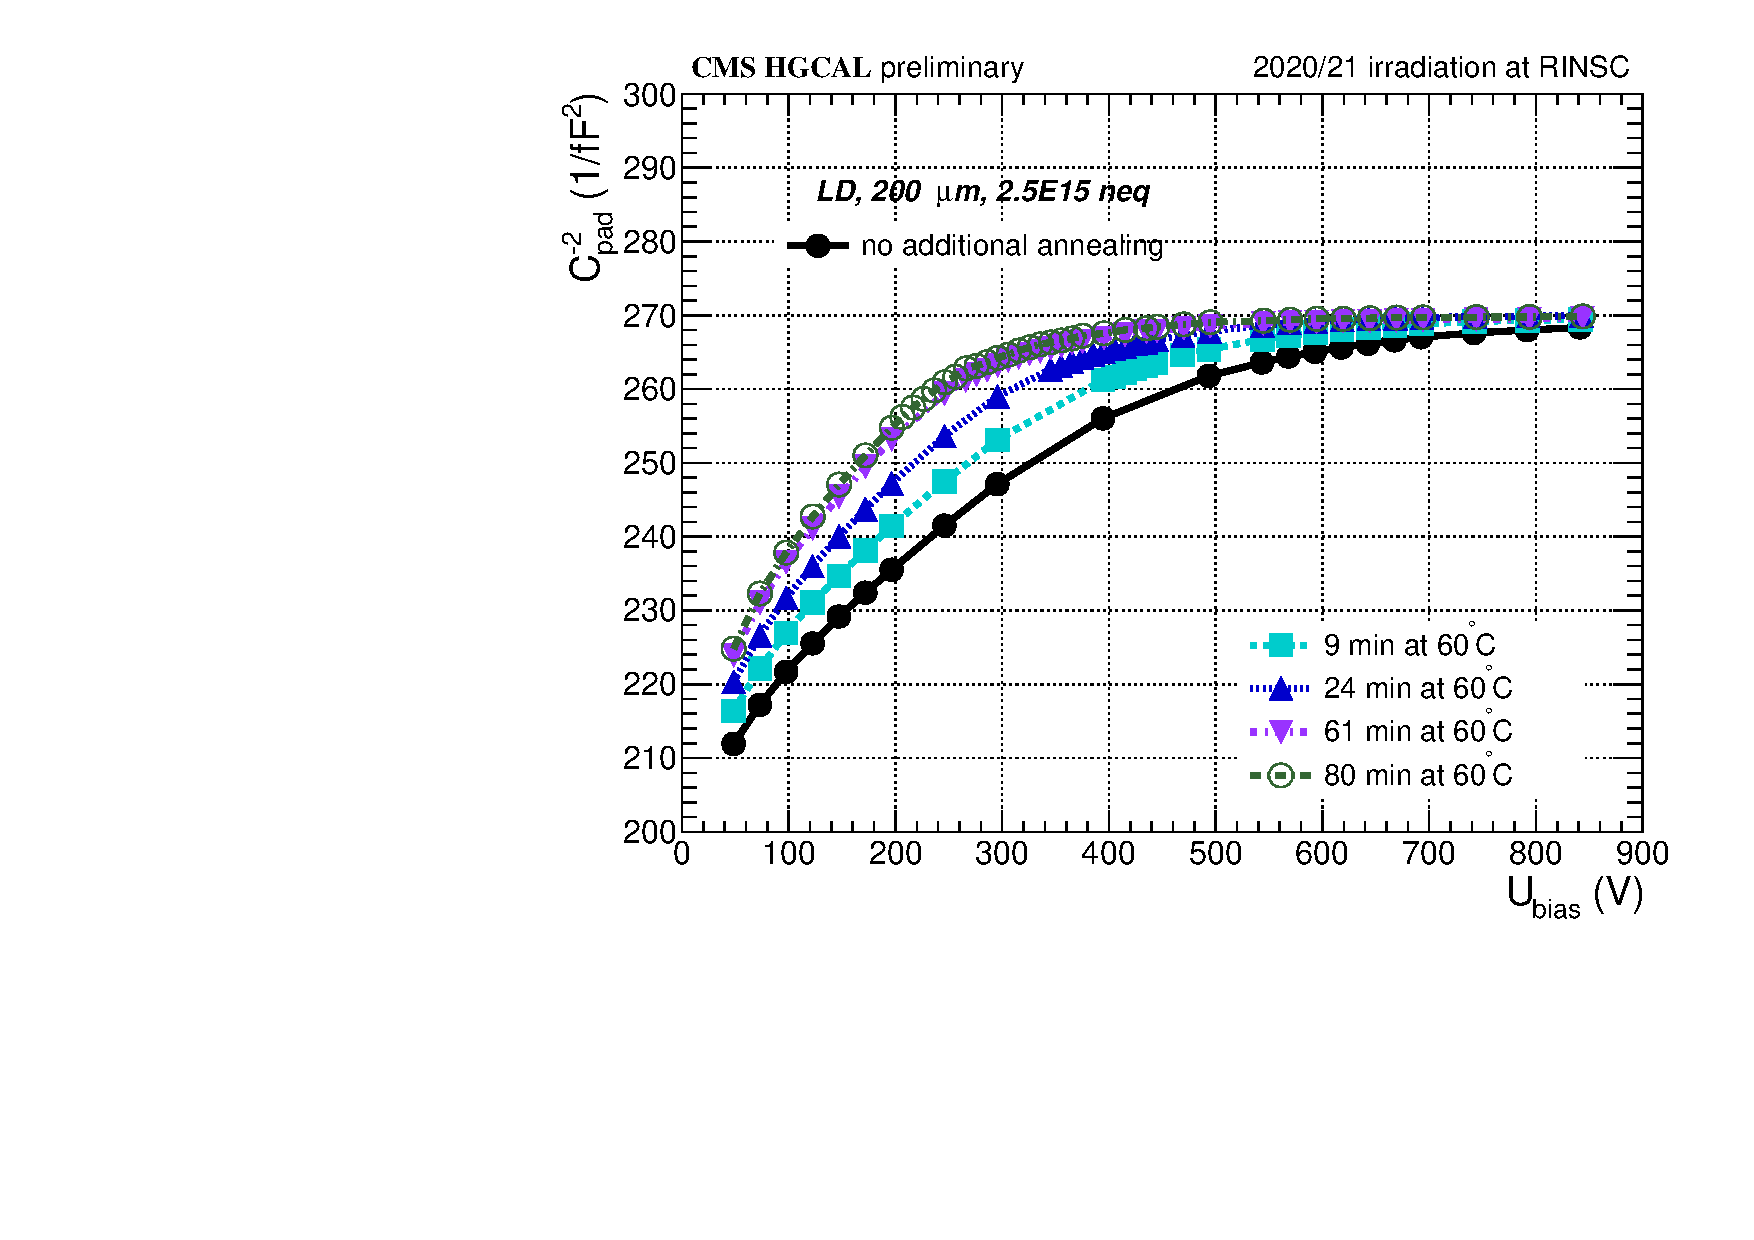
\includegraphics[width=0.999\textwidth]{plots/annealing_Vdep/annealing_CV_ch24.pdf}
		\subcaption{
		}
        \label{plot:annealing_CV}
	\end{subfigure}
    \hfill
    \begin{subfigure}[b]{0.49\textwidth}
		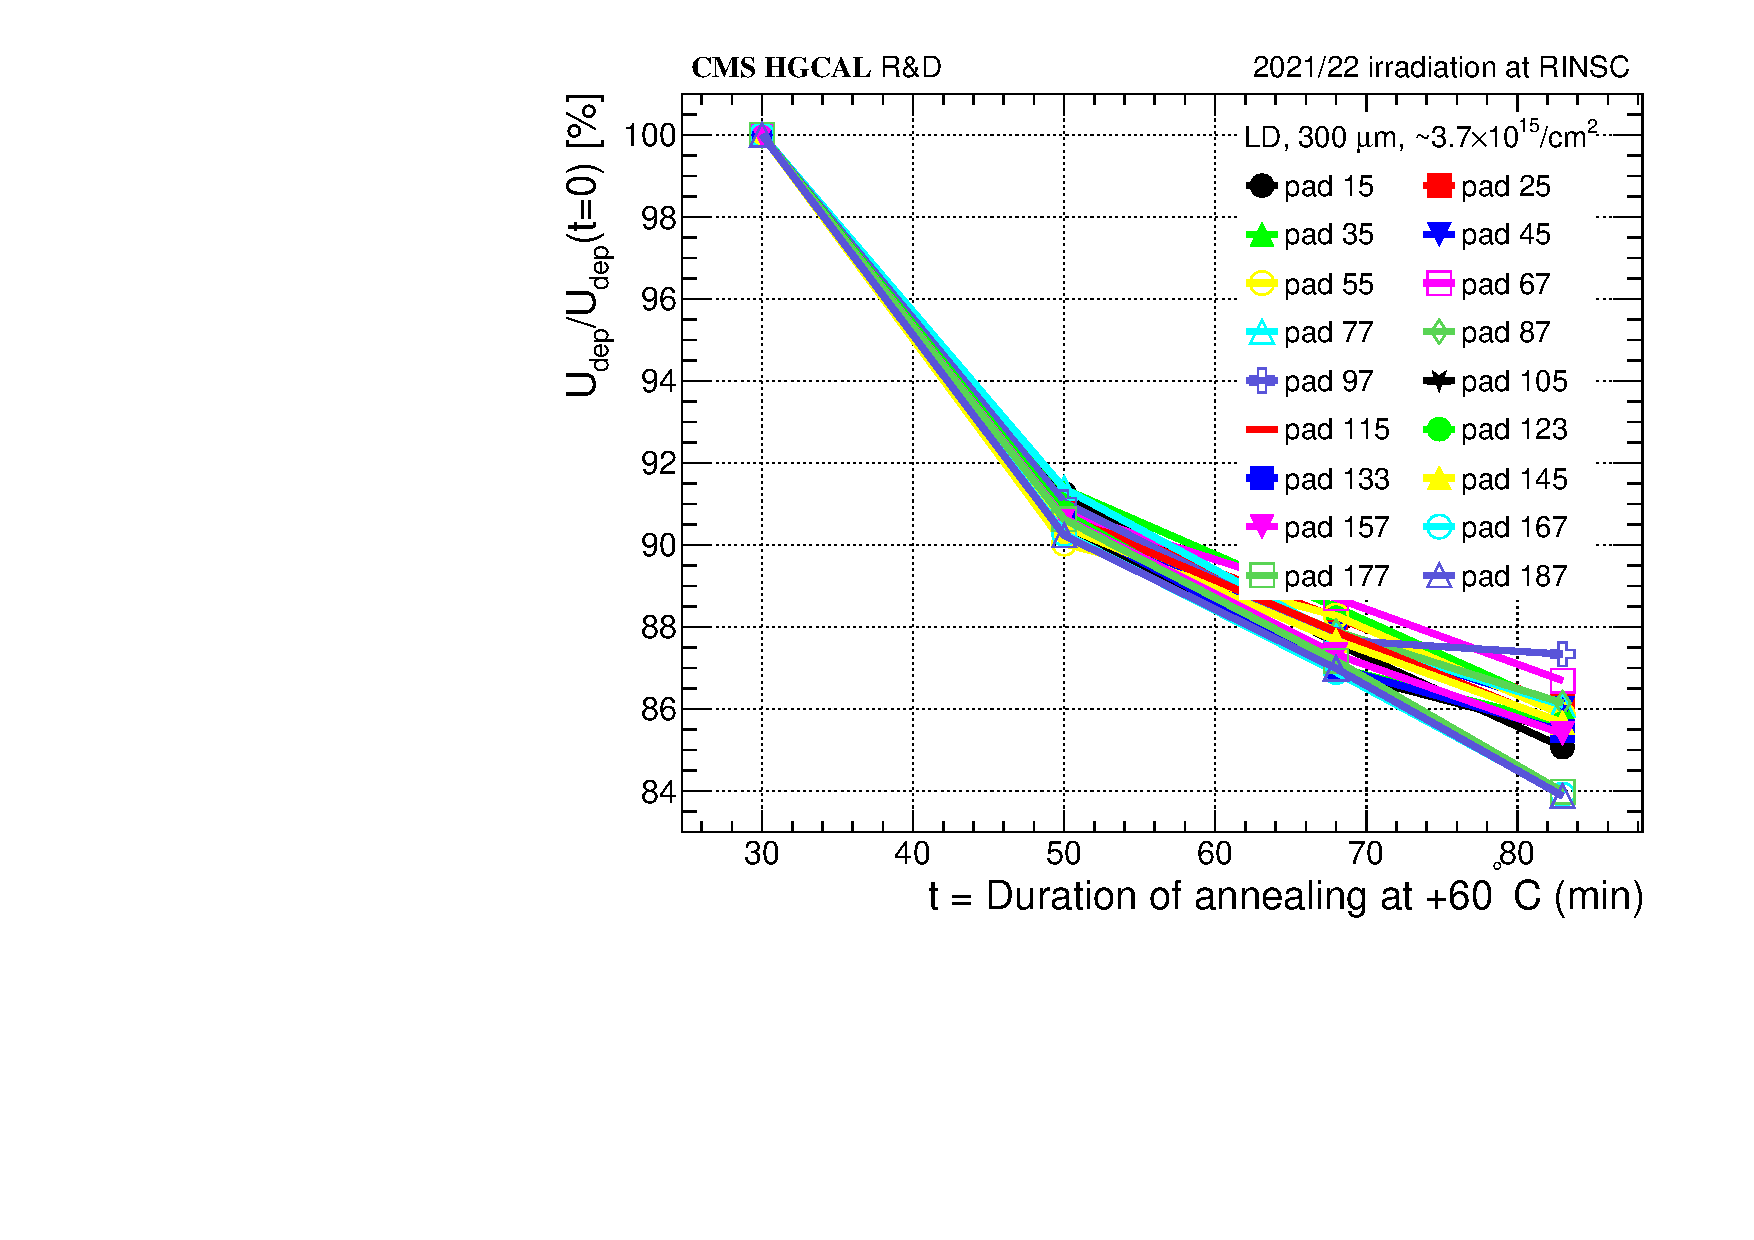
\includegraphics[width=0.999\textwidth]{plots/annealing_Vdep/annealing_Vdep.pdf}
		\subcaption{
		}		
        \label{plot:annealing_Vdep}
	\end{subfigure}
	\caption{
        (a) Inverted CV-curves of a representative full hexagonal pad for different annealing scenarios for a \SI{200}{\micro\metre} low-density prototype sensor irradiated to approximately 2.4$~$E15 1-MeV-neutron equivalents/cm$^{2}$.   
		(b) Relative decrease of the depletion voltage estimate ($U_\text{dep}$) as a function of the additional annealing time at \SI{60}{\celsius} for a subset of full pads.
	}
\end{figure}


\begin{itemize}
	\item Capacitance dominated by bulk, area-normalised capacitance on one sensor = stable within 5 percent, interpad contributions can explain differences?, cf.~\ref{plot:pad_CV_channels}
	\item Depletion voltage, i.e. where final capacitance is reached, clearly differs between fluence scenarios and thicknesses, cf.~\ref{plot:pad_invCV_sensor}, provide table?
	\item Mention inter-pad capacitance from TTU
	\item Depletion voltage hexplot shows profile, matches leakage current profile
\end{itemize}


\begin{figure}
	\captionsetup[subfigure]{aboveskip=-1pt,belowskip=-1pt}
	\centering
	\begin{subfigure}[b]{0.49\textwidth}
		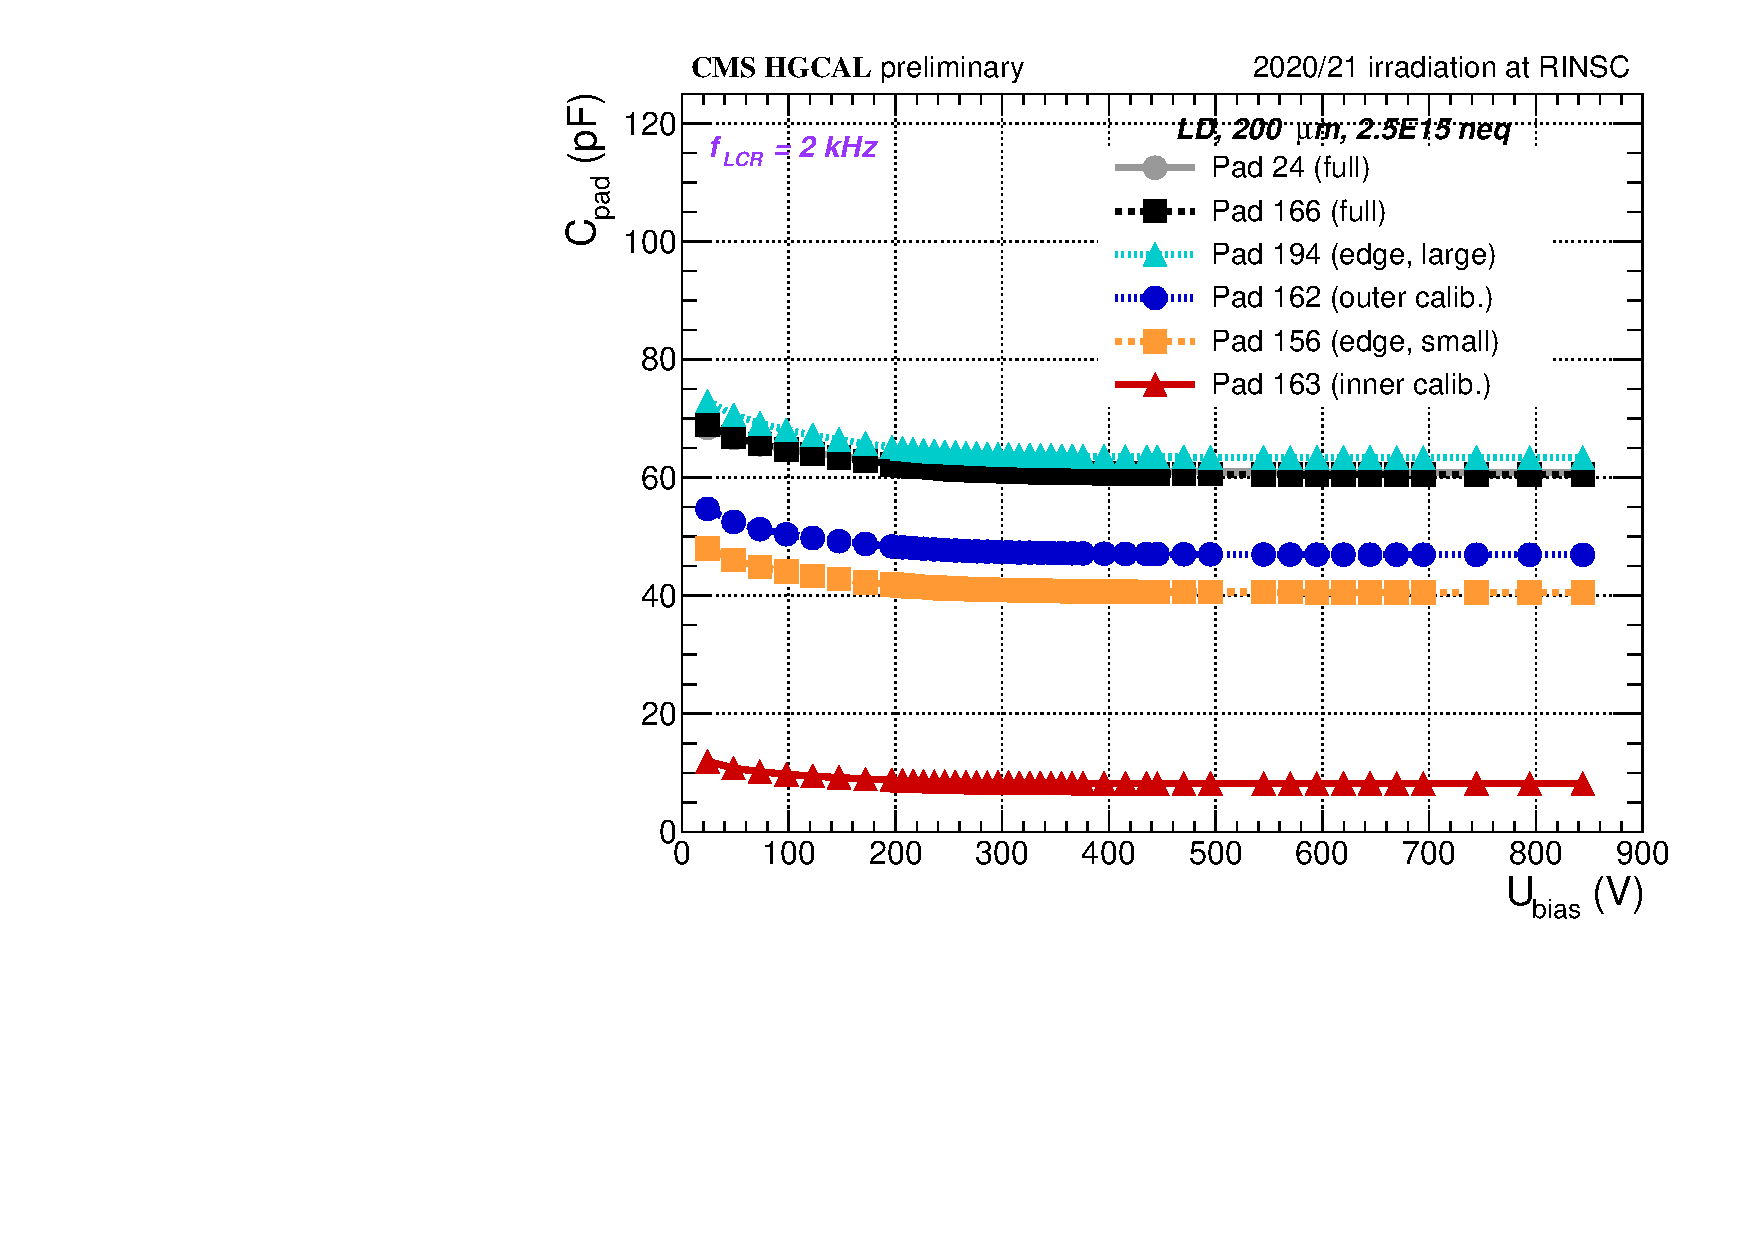
\includegraphics[width=0.999\textwidth]{plots/channel_cv/channel_CV_sensors_channels.pdf}
		\subcaption{
		}
		\label{plot:pad_CV_channels}
	\end{subfigure}
	\hfill
	\begin{subfigure}[b]{0.49\textwidth}
		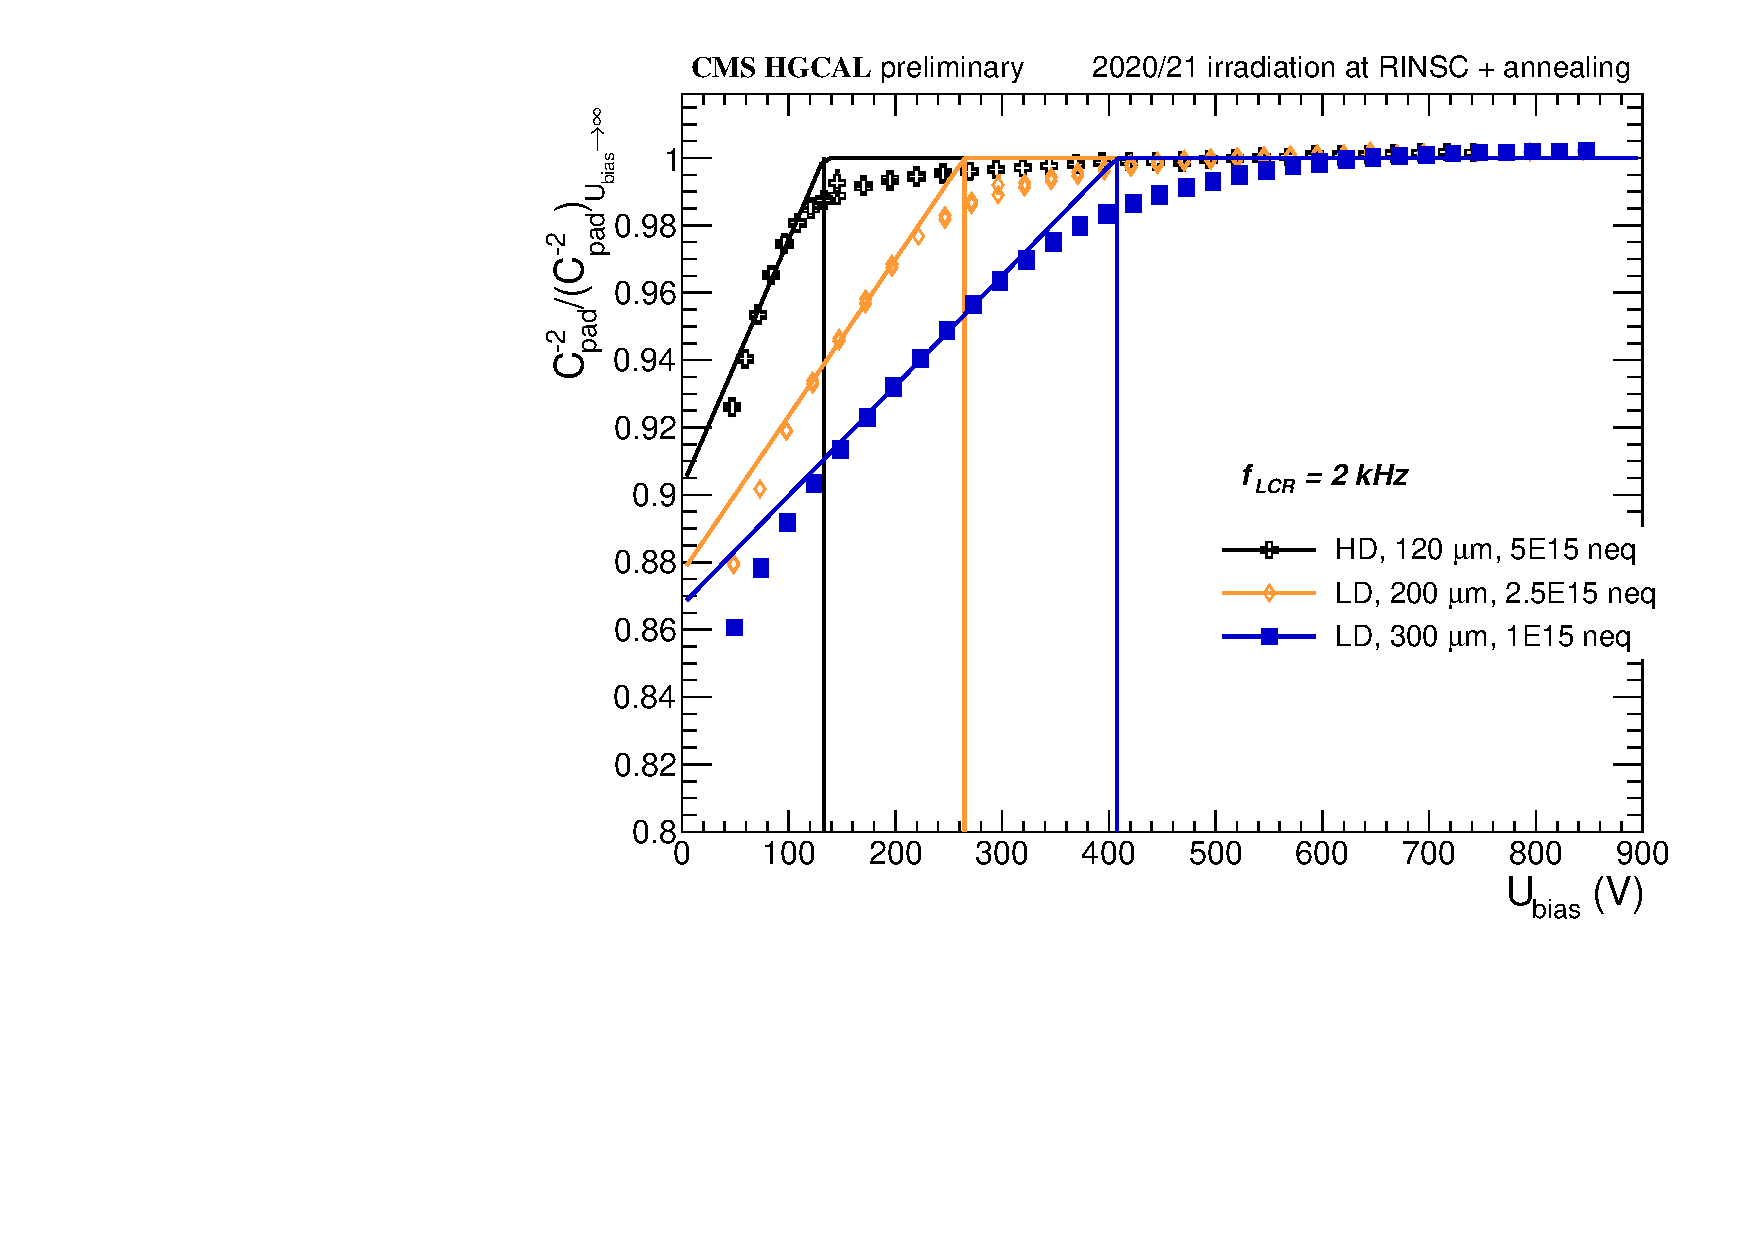
\includegraphics[width=0.999\textwidth]{plots/channel_cv/channel_invCV_sensors_sensors.pdf}
		\subcaption{
		}
		\label{plot:pad_invCV_sensor}
	\end{subfigure}
	\caption{
		(a) Area-normalised capacitances as a function of the effective bias voltage for different pads with different geometries on one example sensor.
		(b) Normalised squared-inverse capacitances as a function of the effective bias voltage for estimating the sensor depletion voltage for one central pad on three example sensors from different irradiation rounds.
		The LCR frequency in these measurements was \SI{2}{\kilo\hertz}.
	}
\end{figure}



\begin{figure}
	\captionsetup[subfigure]{aboveskip=-1pt,belowskip=-1pt}
	\centering
	\begin{subfigure}[b]{0.49\textwidth}
		\centering
		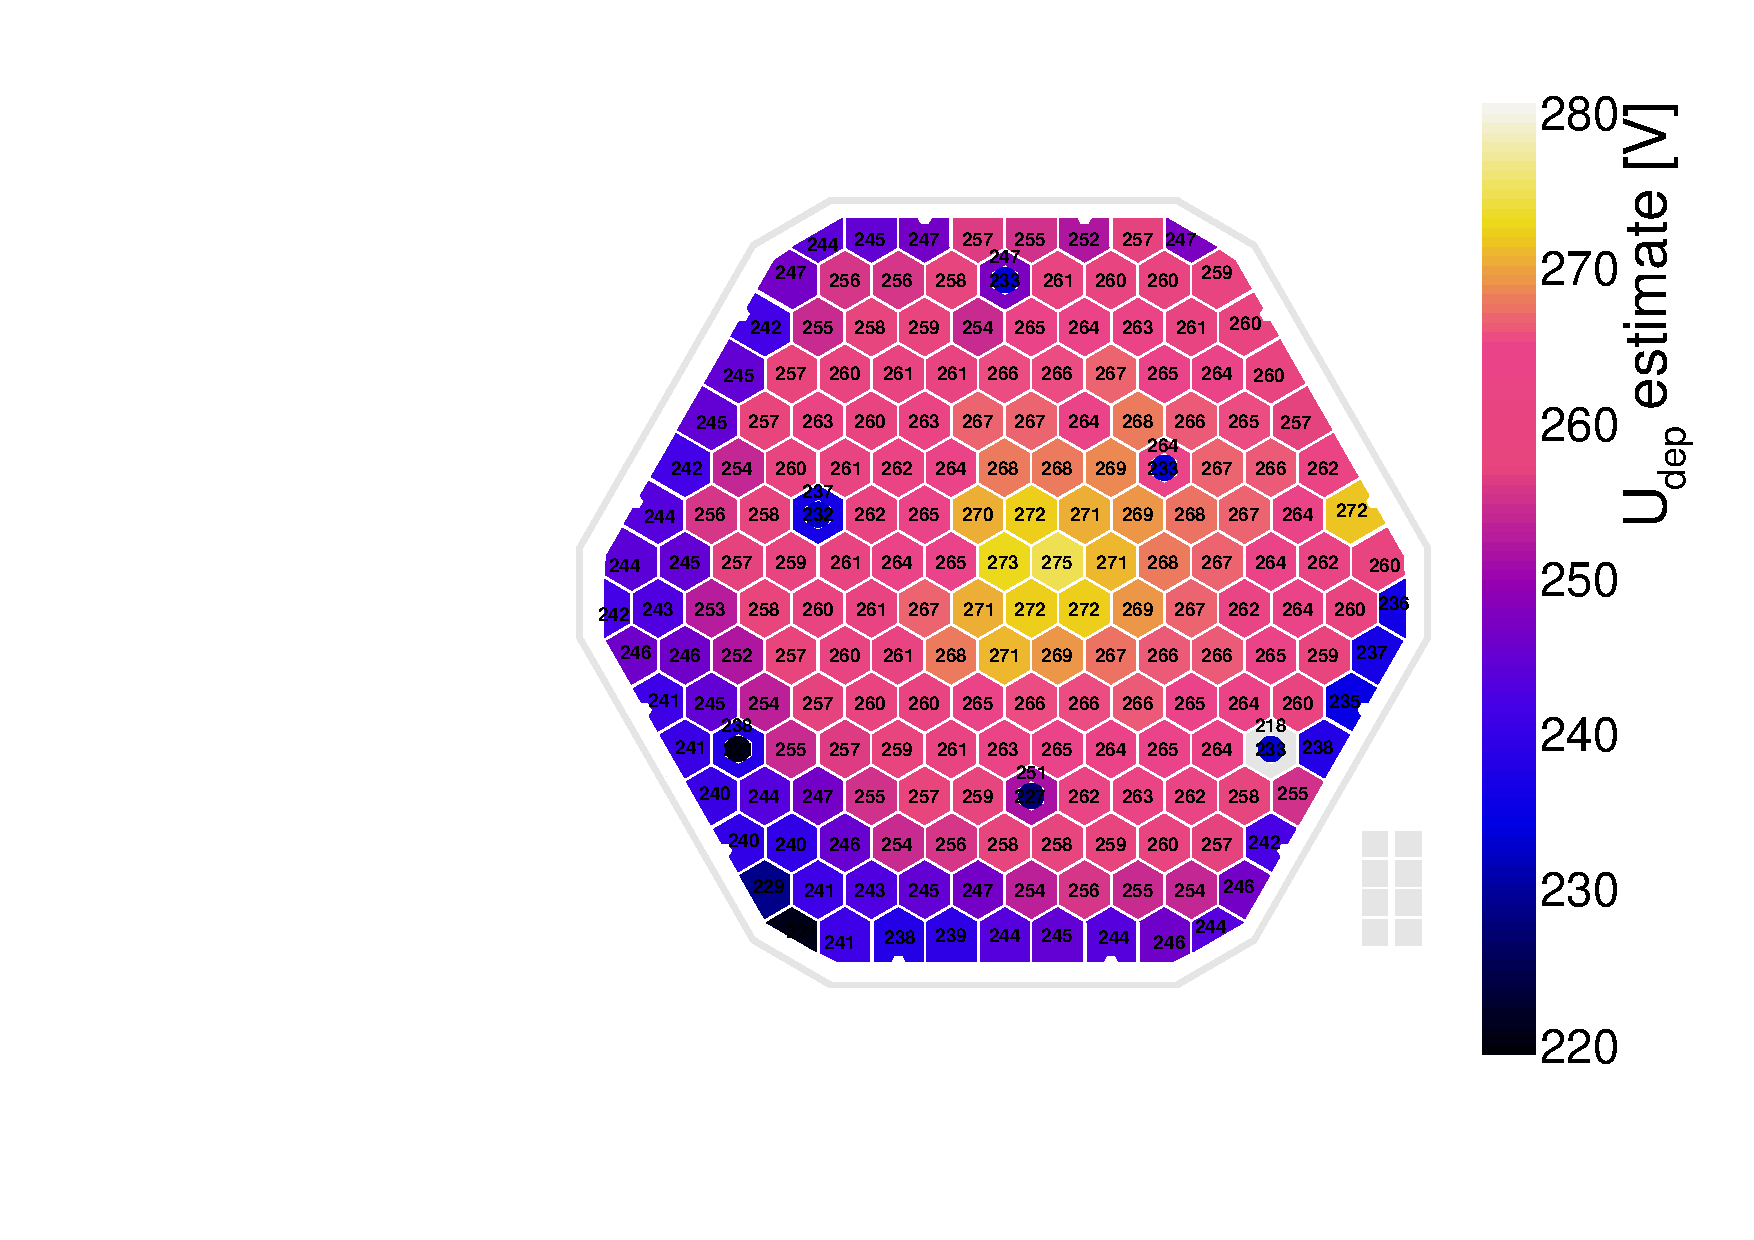
\includegraphics[width=0.99\textwidth]{plots/Vdep_hexplots/0541_04.pdf}
		\subcaption{
			}
			\label{plot:Vdep_hexplot_0541_04}
	\end{subfigure}
	\hfill
	\begin{subfigure}[b]{0.49\textwidth}
		\centering
		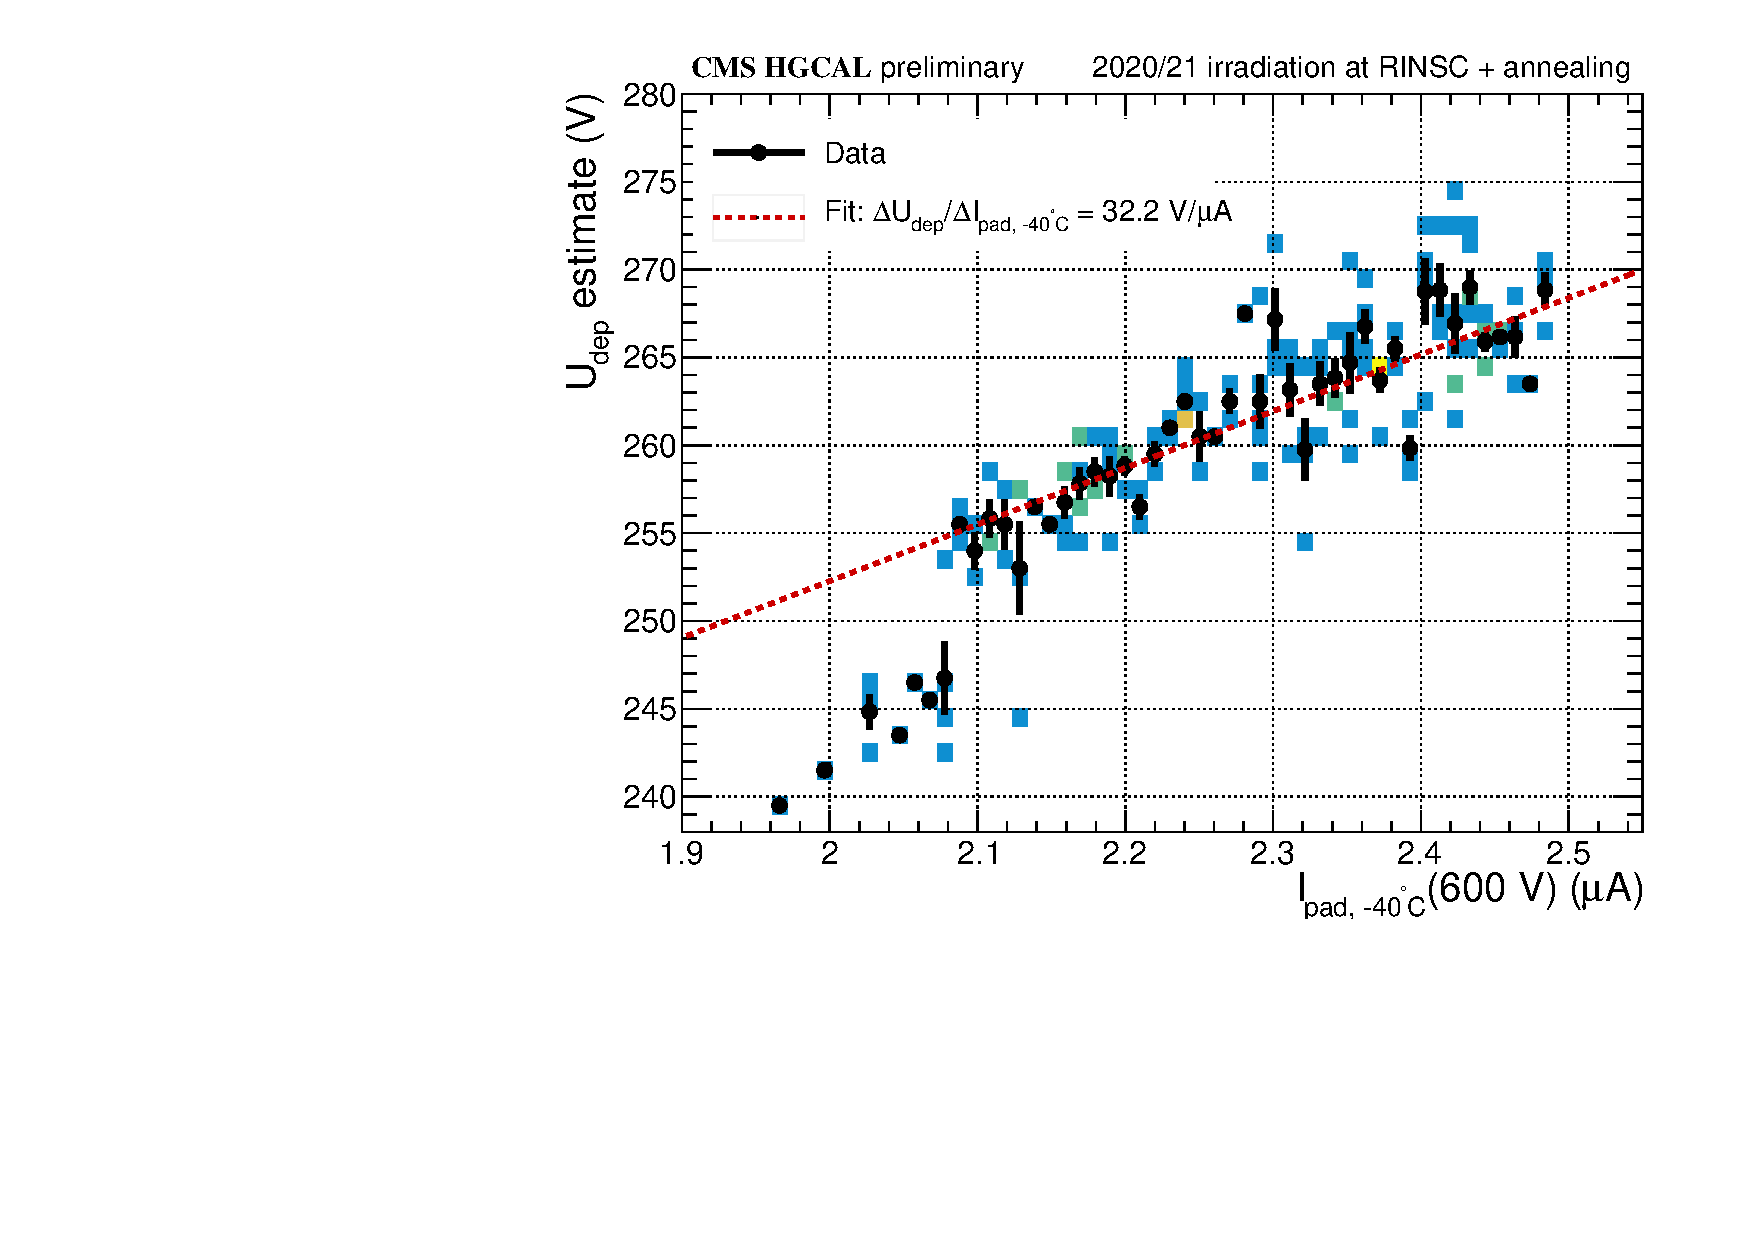
\includegraphics[width=0.999\textwidth]{plots/Vdep_vs_fluence/Vdep_vs_current_5414.pdf}
		\subcaption{
			}
			\label{plot:Vdep_vs_current_5414}
	\end{subfigure}
	\caption{
		(a) Per-pad depletion voltage estimates for a \SI{200}{\micron} LD example sensor irradiated to 1.9E+15$~$neq/cm$^{2}$, and 
		(b) their correlation to the per-pad leakage current, as proxy for the fluence.
	}
\end{figure}

\begin{itemize}
	\item Unlike leakage current: Depletion voltage vs. fluence do not agree between different sensors (as expected). Reason: sizable dependence on production parameters, e.g. active thickness
	\item To test impact of fluence on $U_\text{dep}$: Exploit leakage current profile (taken proportional to fluence profile) to demonstrate positive correlation of depletion voltage to fluence.
	\item Use per-pad leakage current at \SI{600}{\volt} as proxy for fluence
	\item In fact: Observe positive correlation, cf.~\ref{plot:Vdep_vs_current_5414}
	\item Proportionality constant depends on thickness but is consistent between sensors with same thicknesses
\end{itemize}